%%%%%%%%%%%%%%%%%%%%%%%%%%%%%%%%%%%%%%%%%
% Masters/Doctoral Thesis 
% LaTeX Template
% Version 1.42 (19/1/14)
%
% This template has been downloaded from:
% http://www.latextemplates.com
%
% Original authors:
% Steven Gunn 
% http://users.ecs.soton.ac.uk/srg/softwaretools/document/templates/
% and
% Sunil Patel
% http://www.sunilpatel.co.uk/thesis-template/
%
% License:
% CC BY-NC-SA 3.0 (http://creativecommons.org/licenses/by-nc-sa/3.0/)
%
% Note:
% Make sure to edit document variables in the Thesis.cls file
%
%%%%%%%%%%%%%%%%%%%%%%%%%%%%%%%%%%%%%%%%%

%----------------------------------------------------------------------------------------
%	PACKAGES AND OTHER DOCUMENT CONFIGURATIONS
%----------------------------------------------------------------------------------------

\documentclass[11pt, a4paper, oneside]{Thesis} % Paper size, default font size and one-sided paper

\usepackage[T1]{fontenc}
% \usepackage{ebgaramond}
\usepackage{tgpagella}


\graphicspath{{Pictures/}} % Specifies the directory where pictures are stored

\usepackage[square, numbers, comma, sort&compress]{natbib} % Use the natbib reference package - read up on this to edit the reference style; if you want text (e.g. Smith et al., 2012) for the in-text references (instead of numbers), remove 'numbers' 

\usepackage{algorithm}
\usepackage[noend]{algpseudocode}
\usepackage{amsmath}
\DeclareMathOperator*{\argmin}{arg\,min}

\hypersetup{urlcolor=blue, colorlinks=true} % Colors hyperlinks in blue - change to black if annoying
\title{\ttitle} % Defines the thesis title - don't touch this

\begin{document}

\frontmatter % Use roman page numbering style (i, ii, iii, iv...) for the pre-content pages

\setstretch{1.3} % Line spacing of 1.3

% Define the page headers using the FancyHdr package and set up for one-sided printing
\fancyhead{} % Clears all page headers and footers
\rhead{\thepage} % Sets the right side header to show the page number
\lhead{} % Clears the left side page header

\pagestyle{fancy} % Finally, use the "fancy" page style to implement the FancyHdr headers

\newcommand{\HRule}{\rule{\linewidth}{0.5mm}} % New command to make the lines in the title page
\newcommand{\startdescription}{\medskip\small}

% PDF meta-data
\hypersetup{pdftitle={\ttitle}}
\hypersetup{pdfsubject=\subjectname}
\hypersetup{pdfauthor=\authornames}
\hypersetup{pdfkeywords=\keywordnames}

%----------------------------------------------------------------------------------------
%	TITLE PAGE
%----------------------------------------------------------------------------------------

\begin{titlepage}
\begin{center}

\textsc{\LARGE \univname}\\[1.5cm] % University name
\textsc{\Large Bachelor Thesis}\\[0.5cm] % Thesis type

\HRule \\[0.4cm] % Horizontal line
{\huge \bfseries \ttitle}\\[0.4cm] % Thesis title
\HRule \\[1.5cm] % Horizontal line
 
\begin{minipage}{0.4\textwidth}
\begin{flushleft} \large
\emph{Author:}\\
{\authornames} % Author name - remove the \href bracket to remove the link
\end{flushleft}
\end{minipage}
\begin{minipage}{0.4\textwidth}
\begin{flushright} \large
\emph{Supervisor:} \\
{\supname} % Supervisor name - remove the \href bracket to remove the link  
\end{flushright}
\end{minipage}\\[3cm]
 
\large \textit{A thesis submitted in fulfilment of the requirements\\ for the degree of \degreename}\\[0.3cm] % University requirement text
\textit{in}\\[0.4cm]
% \\\deptname\\[2cm] % Research group name and department name
\deptname\\[2cm] % Research group name and department name
 
{\large \today}\\[4cm] % Date
%\includegraphics{Logo} % University/department logo - uncomment to place it
 
\vfill
\end{center}

\end{titlepage}

%----------------------------------------------------------------------------------------
%	DECLARATION PAGE
%	Your institution may give you a different text to place here
%----------------------------------------------------------------------------------------

\Declaration{

\addtocontents{toc}{\vspace{1em}} % Add a gap in the Contents, for aesthetics

% I, \authornames, declare that this thesis titled, '\ttitle' and the work presented in it are my own. I confirm that:
% 
% \begin{itemize} 
% \item[\tiny{$\blacksquare$}] This work was done wholly or mainly while in candidature for a research degree at this University.
% \item[\tiny{$\blacksquare$}] Where any part of this thesis has previously been submitted for a degree or any other qualification at this University or any other institution, this has been clearly stated.
% \item[\tiny{$\blacksquare$}] Where I have consulted the published work of others, this is always clearly attributed.
% \item[\tiny{$\blacksquare$}] Where I have quoted from the work of others, the source is always given. With the exception of such quotations, this thesis is entirely my own work.
% \item[\tiny{$\blacksquare$}] I have acknowledged all main sources of help.
% \item[\tiny{$\blacksquare$}] Where the thesis is based on work done by myself jointly with others, I have made clear exactly what was done by others and what I have contributed myself.\\
% \end{itemize}


\includegraphics[width=\textwidth]{Figures/Declaration.eps}
\vspace{3cm}
 
Signed:\\
\rule[1em]{25em}{0.5pt} % This prints a line for the signature
 
Date:\\
\rule[1em]{25em}{0.5pt} % This prints a line to write the date
}

\clearpage % Start a new page

%----------------------------------------------------------------------------------------
%	QUOTATION PAGE
%----------------------------------------------------------------------------------------

% \pagestyle{empty} % No headers or footers for the following pages
% 
% \null\vfill % Add some space to move the quote down the page a bit

% \textit{``Thanks to my solid academic training, today I can write hundreds of words on virtually any topic without possessing a shred of information, which is how I got a good job in journalism."}

% \begin{flushright}
% Dave Barry
% \end{flushright}

% \vfill\vfill\vfill\vfill\vfill\vfill\null % Add some space at the bottom to position the quote just right
% 
% \clearpage % Start a new page

%----------------------------------------------------------------------------------------
%	ABSTRACT PAGE
%----------------------------------------------------------------------------------------

\addtotoc{Abstract} % Add the "Abstract" page entry to the Contents

\abstract{\addtocontents{toc}{\vspace{1em}} % Add a gap in the Contents, for aesthetics
% The Thesis Abstract is written here (and usually kept to just this page). The page is kept centered vertically so can expand into the blank space above the title too\ldots
Guitar is a musical instrument. Given a guitar score, there exist different fingering alternatives for playing it. It is difficult for novice learners to choose a proper fingering. This thesis describes an application that provides functionalities of sheet music rendering, playing and tablature generating. For sheet music rendering, this thesis describes the procedure from loading musical data from MusicXML file to rendering it to screen. For tablature generation, this thesis proposed a fingering arrangement algorithm using dynamic programming.
For each piece, this fingering arrangement algorithm finds a globally optimal solution in the proposed model. In the proposed model, finger movement including pressing, releasing, moving are considered and their effect are reflected by the cost function. Cost function in this algorithm is rule based and parameters are assigned by experiment. The application has been tested on about 30 guitar pieces and four of them are listed in this thesis.

}

\bigskip
\textbf{Keywords} \\
\keywordnames

\clearpage % Start a new page

%----------------------------------------------------------------------------------------
%	ACKNOWLEDGEMENTS
%----------------------------------------------------------------------------------------

\setstretch{1.3} % Reset the line-spacing to 1.3 for body text (if it has changed)

\acknowledgements{\addtocontents{toc}{\vspace{1em}} % Add a gap in the Contents, for aesthetics
First, to my advisor, A.Prof. Chenying Gao, for the continuous support of the work in this thesis, for her patience, motivation, enthusiasm, and immense knowledge.

Last but not least, I would give my thanks to my family for their permanent understanding and support.

% The acknowledgements and the people to thank go here, don't forget to include your project advisor\ldots
}
\clearpage % Start a new page

%----------------------------------------------------------------------------------------
%	LIST OF CONTENTS/FIGURES/TABLES PAGES
%----------------------------------------------------------------------------------------

\pagestyle{fancy} % The page style headers have been "empty" all this time, now use the "fancy" headers as defined before to bring them back

\lhead{\emph{Contents}} % Set the left side page header to "Contents"
\tableofcontents % Write out the Table of Contents

\lhead{\emph{List of Figures}} % Set the left side page header to "List of Figures"
\listoffigures % Write out the List of Figures

\lhead{\emph{List of Tables}} % Set the left side page header to "List of Tables"
\listoftables % Write out the List of Tables

\listofalgorithms
\addcontentsline{toc}{chapter}{\listalgorithmname}

%----------------------------------------------------------------------------------------
%	ABBREVIATIONS
%----------------------------------------------------------------------------------------

\clearpage % Start a new page

\setstretch{1.5} % Set the line spacing to 1.5, this makes the following tables easier to read

% \lhead{\emph{Abbreviations}} % Set the left side page header to "Abbreviations"
% \listofsymbols{ll} % Include a list of Abbreviations (a table of two columns)
% {
% \textbf{LAH} & \textbf{L}ist \textbf{A}bbreviations \textbf{H}ere \\
% %\textbf{Acronym} & \textbf{W}hat (it) \textbf{S}tands \textbf{F}or \\
% }

%----------------------------------------------------------------------------------------
%	PHYSICAL CONSTANTS/OTHER DEFINITIONS
%----------------------------------------------------------------------------------------

% \clearpage % Start a new page

% \lhead{\emph{Physical Constants}} % Set the left side page header to "Physical Constants"

% \listofconstants{lrcl} % Include a list of Physical Constants (a four column table)
% {
% Speed of Light & $c$ & $=$ & $2.997\ 924\ 58\times10^{8}\ \mbox{ms}^{-\mbox{s}}$ (exact)\\
% % Constant Name & Symbol & = & Constant Value (with units) \\
% }

%----------------------------------------------------------------------------------------
%	SYMBOLS
%----------------------------------------------------------------------------------------

% \clearpage % Start a new page
% 
% \lhead{\emph{Symbols}} % Set the left side page header to "Symbols"
% 
% \listofnomenclature{lll} % Include a list of Symbols (a three column table)
% {
% $a$ & distance & m \\
% $P$ & power & W (Js$^{-1}$) \\
% % Symbol & Name & Unit \\
% 
% & & \\ % Gap to separate the Roman symbols from the Greek
% 
% $\omega$ & angular frequency & rads$^{-1}$ \\
% % Symbol & Name & Unit \\
% }

%----------------------------------------------------------------------------------------
%	DEDICATION
%----------------------------------------------------------------------------------------

\setstretch{1.3} % Return the line spacing back to 1.3

\pagestyle{empty} % Page style needs to be empty for this page

% \dedicatory{For people who enjoy music and guitar.} % Dedication text

\addtocontents{toc}{\vspace{2em}} % Add a gap in the Contents, for aesthetics

%----------------------------------------------------------------------------------------
%	THESIS CONTENT - CHAPTERS
%----------------------------------------------------------------------------------------

\mainmatter % Begin numeric (1,2,3...) page numbering

\pagestyle{fancy} % Return the page headers back to the "fancy" style

% Include the chapters of the thesis as separate files from the Chapters folder
% Uncomment the lines as you write the chapters

\chapter{Introduction}

\label{Chapter:Introduction}
\lhead{\emph{Introduction}}

\section{Background}
Guitar is a popular musical instrument that can be used to play a variety of musical genres.
Typically, a guitar has 6 strings and 17 or more frets, dividing about 100 positions on its fretboard. In this these, we focus on the discussion on classical guitar.
To produce sound with the guitar, one use the fingers on left hand to press a string to the bar on fretboard and pluck this string by right hand.
Without special techniques, each position played by this manner will produce a sound with specific pitch.
Different from the piano, which has a one-to-one correspondence between each pitch and each key on the keyboard, a sound with specific pitch can be produced on different positions on the guitar fretboard.
Therefore, we need to choose some proper positions for the notes that we want to play.

Typical musical scores is written on the five-line staff, from which we can know each note's pitch easily.
The five-line staff is not designed for string instruments so labeling fingering instructions on it
can be cumbersome. For example, once the finger number is labeled around a note, there's no space left for labeling the fretboard position, and vice versa. Scores on many published books has finger names(p, i, m, a, representing four fingers of the left hand) labeled only on the first several measures. In many cases, knowing only the finger names is not enough to finish the fingering arrangement. To describe a complete fingering arrangement, we should assign a fretboard grid and a finger for each note. These make it not easy for beginners to figure out the proper fingering.

Tablature is a form of musical score that solve this problem to some extent.
It's widely used for string instruments.
It adopt a different format to denote music, by telling which position(both string and fret) to use for each note, instead of telling the note's pitch.
However, tablature is not always available. Many guitar pieces have only the score version, especially pieces for classical guitar.
As \citep{constructing-system} mentioned, one reason for this is that once a guitar player become experienced enough, he/she don't need it that much.

\section{Objectives}
The goal of this work is to present an environment for reading, listening and playing the guitar sheet music. Another goal is to provide a library that helps software developers process sheet music. All the source code in this work are open-sourced.

\section{Previous Works}
Sayegh \citep{sayegh1989fingering} proposed the ``optimum path paradigm'' and use dynamic programming on Viterbi network.
Radisavljevic et al.\citep{radisavljevic2004path} proposed a ``path learning'' method to learn the cost function for dynamic programming, from marked data.

D.Radicioni et al.\citep{radicioni2004segmentation} proposed a segment based method, which extended Sayegh's method by adding the segmentation feature.

George et al.\citep{elkoura2003handrix} proposed a more complex model that takes the physical constraints of human hand and guitar fretboard into account. The model is then solved using a greedy algorithm.

\citep{constructing-system} aims to provide a system of fingering arrangement and tablature generation for melodies. This system was designed for melodies, which don't support polyphony music very well.

\section{Contribution}
In this work, we present a sheet music parsing and rendering library and a global optimization fingering arrangement method that supports polyphony music. The final application can read data from MusicXML \citep{good2001musicxml} and then perform the following tasks:
\begin{itemize}
    \item Score rendering.
    \item Tablature generation and rendering.
    \item Sound playing.
\end{itemize}

The novelty of the present work, compared to the previous ones, is that it takes finger pressing, releasing and timing into consideration. The actual time needed for finger movement is considered in the cost functions. The previous works don't take the time between two successive notes into consideration. However, sometimes the timing is important. For example, when the time between two note is long, the player don't have to move the fingers too fast, so we can translate the burdens here in the final arrangement. Since our method is a global optimization method, it can take advantage from the consideration of timing.

Unlike \citep{constructing-system}, the model we proposed for fingering arrangement is designed for polyphony music so than it can be used to nearly all classical pieces.


\section{Structure of this Thesis}
This thesis is divided into three main chapters.

Chapter 2 describes different steps of the sheet processing procedure, from data parsing to the rendering. Finally, some rendering result are put at the end of this chapter.

Chapter 3 is about sound playing. It also help the reader to understand the concept of note sequence, which is also used in Chapter 4.

Chapter 4 first introduces the physical guitar model, and then propose an abstract model for fingering arrangement. It then solves the fingering arrangement problem by the dynamic programming technique. Optimizations are then proposed to improve the time performance of the main algorithm. At the end of this chapter, there are four arrangement results attached and analyzed.

Appendix A lists the instructions for installing the application.
 
\chapter{Processing Sheet Music}

\label{Chapter:Processing-Sheet-Music}
\lhead{\emph{Processing Sheet Music}}

\newcommand{\element}[1]{{\textit #1}}

\section{Introduction}
MusicXML\citep{MusicXML} is a music notation interchange format. Nowadays, most commercial music softwares support this format so we can use it to interchange sheet music between different softwares. Before MusicXML, the universal music notation interchange format is MIDI. However, a midi file don't contains enough information for rendering sheet music. For example, we won't know from midi the direction of note stems. Another example is that a note with specific pitch can be represented differently, with the alternating symbols such as sharp, flat and natural, etc.

As the website of MusicXML states, there are more than 170 applications include MusicXML support. Also, more and more scores in MusicXML format are available in digital music databases. All input data comes from the MuseScore website. 

\section{Parsing MusicXML}
MusicXML, as its name implies, is a XML based format, so we has plenty of libraries in different programing languages available for manipulation.
Though we can use XML libraries to load the XML file, there are still some works to put on the semantic analyzing of the musical content. 
\subsection{Semantic Parsing}
Semantic parsing is a process that converts data from the storage format to internal format.By internal format, we means a format that is easy to use in the application. Since this kind of internal format varies from different application, there are few libraries available for this job. Having such a general library for semantic parsing is actually a reinvention of  a general format. However, MusicXML is already a general format and is intuitive enough so having a new one is not necessary. We explored some open source computer music projects which have MusicXML support and found such internal format. The Music21 library \citep{Music21}  can convert between MusicXML and its own format, but it expose its MusicXML class as public API. The Lilypond \citep{Lilypond} project has a script, namely ``musicxml2ly.py'', for converting from MusicXML to Lilypond's ``.ly'' format. The relevant classes used by this are also not part of the public API and are nearly undocumented, so it's not easy to reuse in our application. Combining these facts, we decide to write our own semantic parser for converting data from MusicXML to a format that can be used other parts of our application, such as rendering, sound playing and fingering arrangement. 

MusicXML is strictly defined by a XML schema, which is also well documented. We can study the file format directly from the schema. In MusicXML, a musical score is stored as a tree structure\footnote{MusicXML has two types: time-wise or part-wise. We discuss only part-wise here}. It has the following main hierarchy, listed from the root: 
\begin{itemize}
    \item score
    \item part
    \item measure
    \item note/rest/direction
\end{itemize}

Before we introduce these element types, one thing worth to mention is that MusicXML use tenths as unit. A tenth is 1 / 10 of the distance between two staff lines.

In the following, we will introduce these element types briefly. More details will be explained when a element is used in the following sections in this chapter.

\subsection{Score}
The score element is the root element. It provides the information about page layout such as page size and page margins. The correspondence of tenths and real world length unit is also specified here.

\subsection{Part}
A part element contains and only contains many measure elements. There may be several parts in a score, however, our implementation only supports one part. This is because most guitar pieces can be expressed using one part and they are actually expressed using only one part. Using one part does not mean that we can't have polyphony music, since MusicXML chords in a single part. This will be explained in \ref{section:measure}.

\subsection{Measure}
\label{section:measure}
The measure element is the most complex part of MusicXML. The most notably elements that it contains are notes, rests and direction. It also contains information about time signature, key signature and tempo.

The timing mechanism inside a measure works by maintaining a time counter with time changing instructions. When a measure is entered, the time counter is set to zero. Then when each note(or rest) is added, the time counter increase the amount of the note's duration. From this aspect, a note's occurrence can be viewed as a time changing instruction. To support polyphony music, we have the ``backup'' and ``forward'' instructions. When a backup Instruction is processed, the time counter decrease an amount stated by the instruction. A forward instruction is processed in a similar way, but make the time counter goes forward instead.

\subsection{Note}
A note element tells us the pitch, duration and display style of the note. Unlike the MIDI format, which represent a pitch by an integer proportional to the logarithm of the physical pitch value, pitch in MusicXML is represented by a (step, octave) pair. A step can be one of (C, D, E, F, G, A, B) and octave is an integer.

A note element also tells about accidentals, dots, stems, beams, etc. Further details will be explained in \ref{section:rendering-sheet-music}.

\subsection{Other Symbols}
There are some other types of symbols on a musical score, such as time signature, key signature, text, etc. These symbols is usually straightforward to handle since they do not depend on each other.

\section{Internal Data Representation}
We adopt a Object Oriented Style in our internal data representation design. As mentioned above, MusicXML has the score-part-measure-note hierarchy. Instead of following the MusicXML hierarchy strictly, we decide to have a sheet-page-measure-note hierarchy. Miscellaneous symbols is attached to measures and notes.
% TODO: class figure here.

One challenge of dealing with MusicXML is that some information is optional, so we need to infer it's default value from the context. For example, the distance of a measure to the measure below it may be omitted, then we need to infer this distance value from the previous measures.. Sometimes we even have to hard code default values in side our application. For example, tempo value is optional in MusicXML. However, without this value we cannot convert the music time to actual physic time.

%TODO: Note

\section{The Parsing Procedure}
In the parsing procedure, a ParseContext is maintained. A ParseContext consist of these values:
\begin{itemize}
    \item sheet: Current sheet.
    \item page: Current page.
    \item measure: Current measure.
    \item beams: A lookup table for beams parsing.
    \item endings: A lookup table for endings parsing, similar to beams.
\end{itemize}

To parse a MusicXML file, we follow the steps below:
\begin{enumerate}
    \item Load the MusicXML schema file.
    \item Load the MusicXML file.
    \item If the file is compressed, decompress it.
    \item Validate the file using the loaded schema.
    \item Initialize the parse context.
    \item Iterate through each measure element in the only part element.
    \item For each measure, if it indicates that a new page should be created, create one.
    \item For each child of the measure node, get the type of this child and use the corresponding handler to handle.
\end{enumerate}

Most of these steps are straightforward: We just read data from the elements and store them to the objects.


\section{Rendering Sheet Music}
\label{section:rendering-sheet-music}

\subsection{Overview}
Sometimes a picture is worth a thousand words. Figure \ref{fig:score-overview} is a overview of the elements on the score. 
\begin{figure}[t]
    \begin{center}
        % \psfig{figure=score-overview}
    \end{center}
    \caption{A sample score for illustration purpose. Elements are highlighted and labeled with names. This sample is rendered by our rendering program and then processed with Inkscape.}
    \label{fig:score-overview}
\end{figure}

The fundamental part of a score are the staff lines. Each group of staff lines are 5 parallel long horizontal lines, forming a grid system for other musical elements. At the beginning of a staff, there's usually a clef followed by the key signature. For guitar pieces, usually the G clef is used. 
A staff is split into measures by the vertical bar lines. A measure helps the reader to group notes and to calculate the time. Each measure has its index number, counting from 0 or 1. It counts from 0 when the measure is partial. Although every measure has an index number, not all of them is printed and usually only the leftmost measure's index number is printed. With the index number, people can describe and locate measures efficiently. 

The vertical bar lines splitting the measures may have different style. They can be thin or thick, single or double. Thin bar line is the most used one. They are used to split measures.
 Thick bar lines are used at the end of a score. Double bar lines, which companied double vertical dots, denote start or end of a repeat.

 Musical notes, along with the stem and beams connecting them, is the most complex part. Details about them will be covered in the following discussion.

\subsection{Primitive Types}
Before we continue on discussing how to render different musical elements, it's worthwhile to classify different primitives.

In musical scores, we only cares about the shape of elements and don't care about the color.So in our model all primitives are rendered using the same color, black.

In our model, all musical elements can be decompose into these 4 primitives:
\begin{itemize}
    \item Lines: Both vertical and horizontal.
    \item Beams: Beams is a special kind of line, with their two ends slanted.
    \item Texture: For example, clefs, quarter note heads, full note heads, tails, rests, accidentals.
    \item Text.
\end{itemize}

A line is actually drawn as a long thin rectangle. Formally, a ``line'' here should be called a segment, since it's not infinite. However, we call it a ``line'' for simplicity's sake.
We use 5 variable to describe a line, they are:
    $$(x_1, y_1, x_2, y_2, \mathrm{thick})$$
This is illustrated by Figure \ref{fig:primitive-line}. One remarkable thing is that we found it important to keep the line ends sharp instead of bevel. This is because bevel ends are hard to align with other elements, causing artifacts in the final render result.

Beams look like lines, except that their ends are slanted. Also, they are attached to the stems most of the time. If we keep using $(x_1, y_1, x_2, y_2, \mathrm{thick})$ to represent a beam, it results that we keep subtracting and adding $\mathrm{thick} / 2$ when calculating
its position. To solve this inconvenience, we use the following representation instead:
\[
    (x_1, y_1, x_2, y_2, \mathrm{height})
\]
The meanings of these variable is illustrated by Figure \ref{fig:primitive-beam}.

To render other elements with irregular shape, we use the template method. First we decompose a complex element symbol into different parts, based on the following rule:
\begin{itemize}
    \item If the symbol has long vertical or horizontal lines, remove it.
    \item For the remaining parts, create a template for each of them.
\end{itemize}
With this method, we get the templates as shown in Figure \ref{fig:primitive-texture}. Since we use OpenGL as the rendering backend, keeping all templates in a single texture image is quite a common way to go. However, packing different templates manually is not easy to maintain, so we make a script using a greedy algorithm to do this. With the help of the script, we can just make each template a single file with its own name, so that we can easily add or remove templates later.

\begin{figure}[t]
    \begin{center}
        % \psfig{figure=primitive-texture}
    \end{center}
    \caption{Packed textures. Each template comes from the Lilypond project. They are rendered into SVG format and then converted to 500dpi PNG image.}
    \label{fig:primitive-texture}
\end{figure}

Each template is represent by:
\[
    (x, y, w, h)
\]
Each template has its pivot point $(x, y)$. This is the coordinate on the final packed image. $w$ stands for ``width'', and $h$ for ``height''. Figure \ref{fig:primitive-example-clef-G} is an example on the G clef about these variables.

\begin{figure}[t]
    \begin{center}
        % \psfig{figure=primitive-example-clef-G}
    \end{center}
    \caption{The G clef template.}
    \label{fig:primitive-example-clef-G}
\end{figure}

Texts are rendering in a similar way like textures.

\subsection{Note}
Notes are the essential part of the score. The pitch of each note is specified by its vertical position and the duration is specified by both its head shape and its tail.

There exists 3 type of note heads. They're for full notes, half notes, and other notes, respectively. Full notes don't have stems connected, and the head is a bit larger than other notes. Half notes looks like quarter notes, except that their heads are hollow. Notes with duration less than quarter has the same note heads, since their duration is then not distinguished by their heads, but their tails instead. As a result, we need to prepare only 3 templates for note head rendering.
 
A note is usually connect by a stem, which heads up or down and has vary length. The direction of a stem is told by MusicXML. Different directions of a stem is used to distinguish between different voice parts. While the head position of a stem is determined by the note head and the stem direction, the tail of it is determined by the beam attached to it, if it has any. A stem without can be any visually proper length. We use 35 tenths as this default value in our application. 

A single stem may be connected to multiple notes. This is often seen in chords. Examples can be found in Figure \ref{fig:score-overview}.

\subsection{Beams}
Beams are used to tell the duration of notes and to group notes. A note \footnote{Here we are discussing notes with quarter note head, since full notes and half notes don't have beams. } without any beams but only a stem have the duration of 1/4. When one more beam is attached, the duration is divided by 2. It's not hard to get the conclusion that a note with $n$ beams have duration of $1 / 2^{n+2}$.

Usually in musical score, beams has different slopes, which is determined by vertical positions of notes that they connect. However, the rules to determine the slope is seldom mentioned. Some software just let the slope be 0. This is, they render all beams horizontally, which make the score look weird and don't comply with the musical convention. 

Here comes three observations that build up the fundamental rules of our method:
\begin{enumerate}
    \item 
        Beams that connected to common stems and have common horizontal span should have the same slope.
    \item
        A proper slope for a beam should make the length of stems connecting to the beam as uniform as possible. 
    \item 
        There should be only several slope value used in rendering, since using too many slope value will mess up the score which is not ideal.
\end{enumerate}


A beam can be partial or complete. Partial beams can then be divided into forward and backward beams. Partial beams cannot occur by it self, since a beam occur by it self is actually a tail, which is rendered differently. With this observation, we can assume that partial beams can always be drawn after complete beams.

A beam may be connected to up stems or down stems, but rarely both. We can assume that all stems that a beam connected to have the same direction. Then we can two types of beam, one with up stems and the other with down stems. Since the calculation between these two types are similar, from this point on we only discuss about the type that has up stems.

In our beam slope calculating algorithm, we have two important concepts:
\begin{itemize}
    \item Length:
the length of a beam is defined as the number of different stems that connected to it. 
    \item Anchor:
        An anchor is a stem that its tail position is determined.
\end{itemize}

Note that if a beam's slope is calculated, the slope of beams below or above it should be the same value. So if we sort the beams by their length, from long to short, and then assign their slope, then we only need to calculate the topmost one in each group of beams. With the aid of anchors, sometimes we can determine the slope of a beam directly. Details is covered in the algorithm listing. \ref{algo:beam-slope}.

\begin{enumerate}
\item Sort the beams by their length, from long to short.
\item For each complete beam, find all anchors connected to it.
\item If the number of anchors is equal or more than 2, then set the beam's left end to the tail position of the leftmost anchor and set the right end to the tail position of the rightmost anchor. Make all stems connected to the beam an new anchor, that is, assign tail position for them. Finish this iteration.
\item Otherwise, sort all stems connected to the beam from left to right.
    % TODO
\end{enumerate}

After this algorithm is performed, we can determine both beam positions and stem positions relative to the measure.

\subsection{Accidentals and dots}
Accidental symbols may occur in two places. The first place is the key signature and the other is the area to the left of note heads. Dots that extending a note's duration may only occur to the right of the note. For accidentals and dots around the note head, it's quite straightforward to render. Once the note's position is determined, we just put them around. 

One remarkable optimization for accidental positioning is that we found a way to avoid the overlap of close accidentals. One situation is illustrated by Figure \ref{fig:avoid-accidental-overlap}. To do this, we first sort all accidentals in a measure, from bottom to top, then left to right. Then we start to put accidentals onto the measure by the sorted order. When an accidental overlap with other ones, move it to left by half of it's width, until there's no overlap. However, to avoid an accidental be moved too far from its original position, we constraint the count of moves to 5 for each accidental. Here the collision detect can use the brute force way, with $O(n^2)$ time complexity, where $n$ is the number of accidentals in the measure. Since there's always only a few accidentals in each measure, this method will work well.

For the accidental symbols used in key signature, there is a set of conventional rules. The writing of key signature is relevant to the clef. Here we only discuss the G clef situation, for the sake of simplicity. In most guitar pieces we only use the G clef.

In MusicXML, the musical key is described by fifths and octave. When the center of G clef is aligned with the second staff line(counting from bottom to top), and if the octave is 3, we know that the second line correspond to the pitch G3. The variable fifths tells about how many fifths we have and what's the accidental type. If fifths is positive, then the type is sharp. If  fifths is negative, then we have flat fifths. For example, if fifths is 1, we know that there is only one sharp, which means the key is G major. If fifths is 2, we know that there are two sharps, and the key is D major.

\subsection{Key Signature}
\subsection{Rendering Order}
\subsection{Different layout Modes}


\section{Playing Sound}

\section{Results}

\chapter{Playing Sound}

\label{Chapter:Playing-Sound}
\lhead{\emph{Playing Sound}}

Sound playing implemented using midi output in our application 

Technically, a piece of music can be treated as a sequence of notes. In our model, a note is described by (pitch, start time, end time).
The pitch format here is different from the pitch format in the rendering engine, which use (step, octave) to describe a pitch.

\section{Pitch Conversion}
We tell the midi output server the notes' pitch by a number ranged from 0 to 255. The standard sound A4, with pitch 440Hz, is represented by 
value 69 in the midi protocol. With this knowledge, we can convert the (step, octave) pair into the midi pitch level by the formula:
\verb|pitchLevel = index('C D EF G A B', step) + octave * 12 - 48 + 60|. Here the ``index(list, element)'' function is used to locate the 
element in the list. For example, index(`C D EF G A B', `C') = 0, index(`C D EF G A B', `E') = 4.

\section{Time Conversion}
Usually, under the musical context, the unit of time is beat. For example, when the time signature is 3/4, it means there are 3 beats in each following
measure and the beat type is quarter beat. To convert to real world time, tempo is needed. Tempo tells us how many beats are there in one minute.
Suppose we have a note with duration equals to $t_d$, and tempo equals to $k$. Then the real world duration can be calculated by:
\[
t_d' = \frac{60 t_d}{k}
\]
The result unit is in seconds. Using this formula, we can accumulate the durations
to get the real world time relative to the beginning of each measure for each note.  

There is another element that can affect the duration of a note's duration. They 
are dots. With a single dot, the duration of a note is multiplied by $1.5$. However, 
with 2 dots, the duration is not multiplied by $1.5^2$. Instead, the result duration 
will be $t_d * (1 + \frac{1}{2} + \frac{1}{2^2})$, where $t_d$ is the origin duration.
Similarly, with $n$ dots, the converted duration will be:
\[
    t_d' = t_d \left(1 + \frac{1}{2} + \frac{1}{2^2} + \frac{1}{2^3} + \cdots + \frac{1}{2^n}\right)
         = t_d \left(2 - \frac{1}{2^n}\right)
\]

\section{Note Sequencing}
To get the final sequence of notes, we need to resolve the repeats in a musical score. At first,
all measures are chained together by in the order of their number. When we start to read a score, 
imagine the there is a cursor put at the beginning of the first measure. As we continue to read,
this cursor starts to move forward. When a end of repeat is encountered, the cursor need to jump back
to the corresponding start of repeat. When this repeat is encountered again, it should be ignored.
An example is illustrated by Figure \ref{fig:repeat-simple}. Sometimes there may be endings come along
with the repeat, this is illustrated by the example in \ref{fig:repeat-with-endings}. Other kinds of repeat
exists such as D.C.al Find(da capo al fine), etc. We will not discuss them here.

\begin{figure}[h]
    \centering
    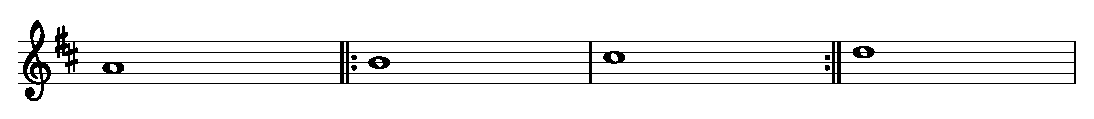
\includegraphics[width=\textwidth]{Figures/repeat-simple.eps}
    \caption{An example for typical repeat.}
    \label{fig:repeat-simple}
    \startdescription
    The read order should be 1,2,3,2,3,4.
\end{figure}

\begin{figure}[h]
    \centering
    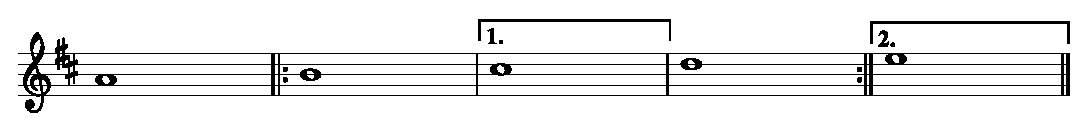
\includegraphics[width=\textwidth]{Figures/repeat-with-endings.eps}
    \caption{An example for repeat with endings.}
    \label{fig:repeat-with-endings}
    \startdescription
    The read order should be 1,2,3,4,2,5.
\end{figure}

% XXX: The flatten algorithm.

\section{Putting All Together}
The midi protocol support two types of event: note\_on and note\_off. We tell the midi server to
start playing a sound with note\_on(pitch, volume, channel) and use note\_off(pitch, volume, channel) to stop
the corresponding sound later. To work with the midi server, we need to convert the node sequence to note events.
Each note will generate exactly two events, one note\_on event and one note\_off event.

In our implementation, each event is described by (event\_type, time, note). To convert from notes to events, we first
generate $2n$ events from the $n$ notes. Then, the events are sorted by their time. Note that there maybe some different
events have the same time. In this case, we use the event type as the comparison key. More specifically, the note\_off event is considered ``less'' than the note\_on event. Otherwise, we are not able to play consecutive notes with same pitch.

The sound playing algorithm is shown in Algorithm \ref{algo:sound-playing}. To make it sound more fluently, we use an extra thread to run the code with implementing algorithm.

\begin{algorithm}
    \caption{Algorithm for Sound Playing} \label{algo:sound-playing}
    \begin{algorithmic}
        \Procedure{play\_sound}{events}
            \Require events sorted by (time, event\_type).
            \State $ t \gets 0$ \Comment{Current time}
            \For{ event $\in$ events}
                \State $ \Delta t \gets \mathrm{event.time} - t$
                \State sleep($\Delta t$)
                \State level $\gets$ convert\_pitch\_level(note.pitch)
                \If {event.type is note\_on}
                    \State note\_on(level, 127, 1)
                \Else
                    \State note\_off(level, 127, 1)
                \EndIf
            \EndFor
        \EndProcedure
    \end{algorithmic}
\end{algorithm}

\chapter{Fingering Arrangement}

\label{Chapter:Fingering-Arrangement}
\lhead{\emph{Fingering Arrangement}}

\section{Introduction}
A guitar consist of several parts. In this problem, we focus on the fretboard only.
Figure \ref{fig:guitar} shows names of the part that we interest about.

\begin{figure}[h]
    \centering
    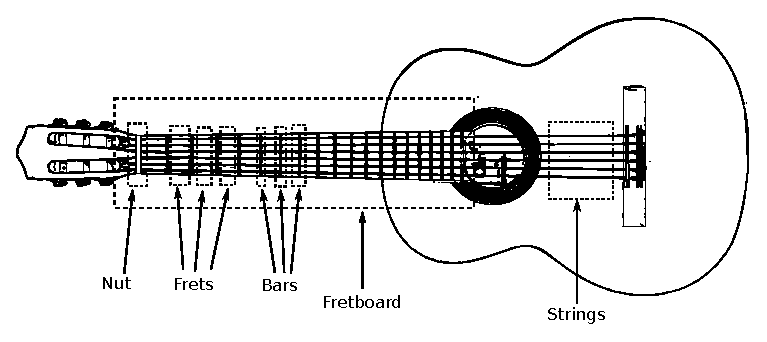
\includegraphics[width=\textwidth]{Figures/guitar.eps}
    \caption{Classical guitar}
    \label{fig:guitar}
\end{figure}

The fretboard can be viewed as a grid system split by 6 strings and 17(or more) bars. For consistence, we assume there is 17 bars on the fretboard. A grid can be described by the (fret, string) pair, where fret ranges from 0 to 17 and string ranges from 0 to 5. The frets count from left to right in Figure \ref{fig:guitar}, and strings count from top to bottom.

When playing the guitar, one use the left hand to press a grid, then use right hand to pluck the corresponding string, then a sound can be produced. Some sounds can be produced by plucking the string without pressing the grid since all strings are attached to the nut. This is so-called ``play by empty string''. We consider fret 0 is used in the empty string situation.

Four fingers in ones left hand are used for pressing the fretboard. Thumb is not used in this job, it is used to grip the neck of guitar. In our discussion, fingers of left hand are numbered into 0, 1, 2, 3, where 0 is for the index finger, and so on. A single finger can press only one grid at a time, except the index finger. We can use the index finger to press more than one grid at a time. This technique is called ``baring''. It cannot be used in every combination of grids. Instead, it can only be used to press the grids on the same fret and a consecutive range of strings. Figure \ref{fig:fretboard-baring} shows an example of the baring technique.

\begin{figure}[h]
    \centering
    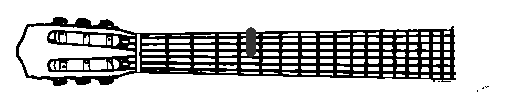
\includegraphics[width=0.6\textwidth]{Figures/fretboard-baring.eps}
    \caption{Baring by the index finger.}
    \label{fig:fretboard-baring}
    \startdescription
    In this example, fret 5 of strings (0, 1, 2) is pressed by the index finger.
\end{figure}

Normally, without special techniques, each grid on the fretboard can only produce a specific
pitch of sound. For example, The grid (5, 0) can produce sound A4(440Hz) and grid (1, 0) can produce C4. Table \ref{table:standard-tuning} shows the pitch that can be produced by each grid on the fretboard. From this table we see that the pitches on the same string are ascending uniformly. Once the pitch of grid (0, $i$) is known to be $p_i$, the pitch of grid ($f$, $i$) can be calculated by $p_i + f$.

\begin{table}
    \centering
    \tiny \tabcolsep=0.05cm
\begin{tabular*}{\textwidth}{r|c|c|c|c|c|c|c|c|c|c|c|c|c|c}
& 0& 1& 2& 3& 4& 5& 6& 7& 8& 9& 10& 11& 12& 13\\ \hline
0
& E4(64)& F4(65)& F\#4(66)& G4(67)& G\#4(68)& A4(69)& A\#4(70)& B4(71)& C5(72)& C\#5(73)& D5(74)& D\#5(75)& E5(76)& F5(77)\\ \hline
1
& B3(59)& C4(60)& C\#4(61)& D4(62)& D\#4(63)& E4(64)& F4(65)& F\#4(66)& G4(67)& G\#4(68)& A4(69)& A\#4(70)& B4(71)& C5(72)\\ \hline
2
& G3(55)& G\#3(56)& A3(57)& A\#3(58)& B3(59)& C4(60)& C\#4(61)& D4(62)& D\#4(63)& E4(64)& F4(65)& F\#4(66)& G4(67)& G\#4(68)\\ \hline
3
& D3(50)& D\#3(51)& E3(52)& F3(53)& F\#3(54)& G3(55)& G\#3(56)& A3(57)& A\#3(58)& B3(59)& C4(60)& C\#4(61)& D4(62)& D\#4(63)\\ \hline
4
& A2(45)& A\#2(46)& B2(47)& C3(48)& C\#3(49)& D3(50)& D\#3(51)& E3(52)& F3(53)& F\#3(54)& G3(55)& G\#3(56)& A3(57)& A\#3(58)\\ \hline
5
& E2(40)& F2(41)& F\#2(42)& G2(43)& G\#2(44)& A2(45)& A\#2(46)& B2(47)& C3(48)& C\#3(49)& D3(50)& D\#3(51)& E3(52)& F3(53)\\ \hline
\end{tabular*}
    \caption{Fretboard pitch table on standard tuning}
    \label{table:standard-tuning}
    \startdescription
    Number in the parentheses are the midi pitch level.
\end{table}

The problem of fingering arrangement is to assign a grid and a finger for each desired notes that we want to produce. 

In Table \ref{table:standard-tuning}, we can see that different grids may produce same pitch. For example, both grids (5, 5) and (0, 4) can produce A2, and both grids (1, 1), (5, 2), (10, 3), (15, 4) can produce C4. Actually, almost every pitch can be produced by more than one grid. Also, different grids can be pressed by different fingers. All these make it impractical to  enumerate all possible combinations to find the optimal solution. By optimal we mean the one that is most easy to play. This will be defined formally in the next section.

\section{Model}
In this problem, we describe a note by (pitch, start time, end time). The solution to the problem should resolve each note by assigning a (finger, fret, string). Since a note can also be played by empty string, the finger value in (finger, fret, string) tuple may equal to -1, which means no finger. 
\[
\mathrm{fingerings} \gets \mathrm{Arrange}(\mathrm{noteSequence})
\]

\subsection{Key Times}
A key time is a time that one or more notes start. Key times are important because all the finger movements start at key time. The first step to solve this problem is to extract all start times from the note sequence as the key time collection. The key time collection is a sequence of different key times.

\subsection{Frame}
A frame at time $t$ is defined as the collection of notes whose time interval contains $t$. More formally, suppose the note is represented by $(p, t_1, t_2)$, and the note sequence is denoted by $N$, then the frame is \[
\mathrm{frame(t)} = \left\{ (p, t_1, t_2) | (p, t_1, t_2) \in N, t_1 \le t < t_2 \right\}
\]
In our method, only frames at key times are interested. All frames are generated by a scanning algorithm, which is described in Algorithm \ref{algo:gen-frames}. First we convert the notes into note events, as we do in chapter \ref{Chapter:Playing-Sound}. Then during the scanning process, we use a list to keep track of the active note events. At time $t$, from the active events we know the notes in the current frame.

\begin{algorithm}[h]
    \caption{Generate Frames} \label{algo:gen-frames}.
    \begin{algorithmic}
        \Function{Generate Frames}{$T$, $E$} \Comment{$T$ is the key time sequence. $E$ is the note event sequence.}
            \Require $E$ is sorted by start time.
            \State F $\gets$ empty set \Comment{The frame sequence.}
            \State $E_a$ $\gets$ empty list \Comment{Active events.}
            \State $p \gets 0$
            \For {$t \in T$}
                \State $E_a \gets \left\{e | e \in E_a, e.\mathrm{end} > t \right\}$
                \While {$p < \mathrm{length}(E)$ and $E(i).\mathrm{start} == t$}
                    \State Append $E(i)$ to $E_a$
                    \State $p \gets p + 1$
                \EndWhile
            \EndFor
            \State make a frame using $E_a$ and then append it to $F$
            \State \Return $F$
        \EndFunction

    \end{algorithmic}
\end{algorithm}

\subsection{Play State}
A play-state at time $t$ describes the state of the left hand and the ringing strings. With these information, we will be able to calculate the cost at time $t$ or cost between two successive key time.

A play-state can be represented by \[ (b, F(i), S(i), R(j)) \] Where $b$ tells this state is barring or not; $F$ and $S$ are functions and their domain is the finger collection ${0, 1, 2, 3}$. In this state, finger $i$ is pressing the grid $(F(i), S(i))$. $R$ is also a function and its domain is the string collection ${0, 1, 2, 3, 4, 5}$. $R(j) = \mathrm{True}$ means that in this state, string $j$ is used.

In our method only play-states at key times are interested. 
A valid play-state for time $t$ is  a play-state that can produce all notes in $\mathrm{frame}(t)$. At each key time, we may have multiple valid play-states.  The solution of the fingering arrangement problem can be described by a sequence of play-states. In such a solution, a play-state is chosen for each key time. 

Suppose in a solution, play-state $S_i$ is assigned to the $i$-th key time $t_i$. Since a play-state tells us all information about how to put the left hand, knowing $S_i$ and $S_{i+1}$ is sufficient to let the player move the left hand. The cost at all play-state $S_i$, and between all $S_i$, $S_{i+1}$ pairs, are summed up to get the total cost for this solution, using equation \ref{eqn:solution-cost}.
\begin{eqnarray}
    & \mathrm{SolutionCost}(
        \left\{t_0, t_1, \cdots, t_n\right\}, \left\{S_0, S_1, \cdots, S_n\right\}
    )  \nonumber\\
    =& \sum_{i = 0}^n C_{\mathrm{static}}(S_i)
    + \sum_{i = 0}^{n - 1} C_{\mathrm{transition}}(t_i, t_{i+1}, S_i, S_{i+1})
    \label{eqn:solution-cost}
\end{eqnarray}

The cost functions $C_{\mathrm{static}}(S_i)$ and $C_{\mathrm{transition}}(t_i, t_{i+1}, S_i, S_{i+1})$ will be discussed in section \ref{section:cost-function}.

\subsection{State Transition Equation}
We use a dynamic programming method to find the play-states solution. 

Let $C(t_i, S)$ be the minimum cost to stay at play-state $S$ at key time $t_i$. Then we can calculate $C(t_i, S)$ using dynamic programming.
All valid play-state for each frame is generated before we calculate $C(t_i, S)$.  We denote the valid play-state for frame at time $t_i$ as $V_i$.

\begin{eqnarray}
    C(t_i, S) = C_{\mathrm{static}}(S) +
        \min_{S' \in V_{i-1}} \left[
            C(t_{i-1}, S') + 
            C_{\mathrm{transition}}(t_{i-1}, t_i, S', S) 
        \right]
    \label{eqn:transition}
\end{eqnarray}
Our goal is to find the play-state $S$ such that $C(t_n, S)$ has the minimum value. Once we got such an $S$,  we can trace back the play-state sequence by the decision on every step to get the corresponding play-state sequence. 


\section{Generating Valid play-state}
A play-state is considered valid if and only if it's playable. Human hand has physical constraint, so some of the grid combinations are impossible to play. Suppose we now have a play-state $S=(b, F(i), S(i), R(j))$, the constraints are listed below.
\begin{enumerate}
    \item For any $i, j, i \le j$, we have $F(i) \le F(j)$.
    \item For any $i, j, i \neq j$, we have $S(i) \neq S(j)$.
    \item For any $i, j, i \le j \land F(i) = F(j)$, we have $S(i) > S(j)$.
    \item When $b = True$, then for any $i > 0$, we have $F(i) > F(0)$.
    \item Fingers should not be too far away from index finger.
    \item When $b = True$, fingers should not be too close from index finger.
\end{enumerate}

Here we set the constraint distance value to maximum or minimum distance that our hand can stretch. The values we used in our implementation are listed in Table \ref{table:finger-constraints}.

\begin{table}[h]
    \centering
    \begin{tabular}{r|r|r|r}
        Fingers & 1 & 2 & 3 \\
        \hline
        max & 0.06 & 0.10 & 0.13 \\
        min & 0.008 & 0.025 & 0.025 \\
    \end{tabular}
    \caption{Finger constraint distance values(in meters).}
    \label{table:finger-constraints}
\end{table}

To calculate the distance between any two grids, we need to know every bar positions. A guitar produces sound by the vibration of strings. When a string is pressed onto the fretboard, its length that contribute to the sound generation is effectively shortened. The frequency of the sound that a string produced is proportional to the multiplicative inverse of the effective length of the string. From the design of guitar, we know that the position of the 12th bar is in the exactly middle of a string. If the length of a string is $L$, then the distance $d_i$ of the $i$-th bar can be calculated by solving equations \ref{eqn:fretboard-proportional}.
\begin{eqnarray}
    \left\{
    \begin{aligned}
        l_i &=  L - d_i \\
        l_{12} &=  L - \frac{L}{2} \\
        l_i p_i &=  l_{12} p_{12} \\
        p_i &=  p_{12} (\sqrt{2})^{ \frac{i}{12}}
    \end{aligned}
    \label{eqn:fretboard-proportional}
    \right.
\end{eqnarray}

Solving these equations we got \[ d_i = (1 - 2^{-i/12})L \]
With this formula we can calculate the distance of any pair of grids.

To generate all valid states for a frame efficiently, we use the strategy that removes the invalid states as early as possible. First, the fret for index finger is chosen. With the index finger chosen, the remaining search space become much smaller. Then we choose to use the index finger or not. Even if the index finger is not used, the fret position of it can describe the hand position. If the index finger is used, a string will be assigned to it. After these steps, the search space is small enough so we can use a brute force recursive searching method to resolve the remaining notes.At each level of recursion, we resolve a note at current frame, and then test the validness according to the constraints. If all the notes are resolve at some level, we start to assign fingers to the used grids. Finally, a new valid play-state is generated.

\section{Cost Function} \label{section:cost-function}
We have two types of cost functions. The first type is the static cost function. The other type is transition function. Static cost is only relevant to frame and play-state at a single key time, while transition cost is relevant to two key times. 

\subsection{Static Cost}
Static cost function consists of two parts: the ``missing penalty'' and the ``high fret penalty''. Missing notes in a play-state is heavily penalized. A note is considered missing in a play-state when it's not resolved by the state. In Figure \ref{fig:guitar}, we can see that frets higher than the 12th bar is on the front surface of the guitar. This make it more difficult to use the frets there, because there's no place for the thumb to grip the neck(it's out of the neck!). Therefore, we have penalty on high frets. In our implementation, fret higher than 9 are considered high. Summarizing these two types of cost, and suppose play-state to be $(b, F, S, R)$  we get:
    \[
    C_{\mathrm{static}}(S) = n_{\mathrm{miss}} K_{\mathrm{miss}} 
        + \sum_{F(i) > F_{\mathrm{high}}} (F(i) - F_{\mathrm{high}}) K_{\mathrm{high}}
    \]
Where $K_{\mathrm{miss}}$ and $K_{\mathrm{high}}$ are constants we got by experiment. 

\subsection{Transition Cost}
Transition cost describes the cost when the hand translates from one state to another state. It can be calculated by summing the movement cost of the arm and the movement cost of each finger. Suppose we are to calculate $C_{\mathrm{transition}}(t_1, t_2, S_1, S_2)$.
The predicate function $P(S, i)$ tells if finger $i$ is pressed in play-state $S$. Then, for finger $i$ from fingers other than index, we observe these 4 situations: 
\begin{description}
    \item[$\lnot P(S_1, i) \land \lnot P(S_2, i)$] \hfill \\
        A free transition, finger $i$ is not used in both play-state. No cost to add.

    \item[$\lnot P(S_1, i) \land P(S_2, i)$] \hfill \\
        Finger $i$ need to pressed on the grid $(F_2(i), S_2(i))$ before time $t_2$. From $S_1$ we can know that when should string $S_2(i)$ stop, then we can calculate the time $\Delta t$ the finger can use to press.
        Add $K_{\mathrm{press}} / \Delta t$ to total cost.

    \item[$P(S_1, i) \land P(S_2, i)$] \hfill \\
        The finger is pressing some grid in both states. Note that the grids it press may be the same or different. If they are the same, add $K_{\mathrm{keep}}(t_2 - t_1)$ to total cost. If they are different, the finger is moved from grid $(F_1(i), S_1(i))$ to $(F_2(i), S_2(i))$,
        so we add \[
        K_{\mathrm{movefret}} \left[ (F_1(i) - F_1(0)) - (F_2(i) - F_2(0)) \right]^2
        + K_{\mathrm{movestring}} \left( S_1(i) - S_2(i)\right)^2
        \]

    \item[$P(S_1, i) \land \lnot P(S_2, i)$] \hfill \\
        Finger $i$ should be released before time $t_2$. The time interval $\Delta t$ that the finger can use to release is calculated similar to the one we use to calculate pressing time. Add $K_{\mathrm{release}} / \Delta t$ to total cost.
\end{description}

For the index finger, which has three states, the cost calculation is similar, but a bit more complexed. It has 9 situations but some are overlapped with the normal fingers'. We are not going to list them here.

One other cost is the missing penalty. If a note is in both frames at $t_1$ and $t_2$, and is resolved by different grid or finger, then this note is considered missing. This is because we cannot keep the string vibrating when switching to another finger. This kind of missing is also penalized by
$n_\mathrm{miss} K_\mathrm{miss}$.


\section{Decision Process}

From equation \ref{eqn:transition}, we can see that once we know all $C(t_{i-1}, S')$ for any 
$S'$, we are able to calculate $C(t_i, S)$. $C(t_0, S)$ is calculated by taking only the static cost.
Using math induction, we can calculate $C(t_n, S)$ for any $S$. Finally we got Algorithm \ref{algo:dp}

\begin{algorithm}
    \caption{Calculate Cost} \label{algo:dp}
    \begin{algorithmic}
    \Procedure {Calculate Cost}{$T$, $F$}
        \State \Comment{$T$: key times, $F$: key frames}
        \State Generate valid states $V_i$ for each frame $F_i$.
        \State D $\gets$ empty table \Comment Choice table
        \State C $\gets$ empty table \Comment Cost table
        \For {$S \in V_0$} 
            \State $C(t_0, S) \gets C_{\mathrm{static}(S)}$
        \EndFor
        \For {$i \in [1, n]$}
            \For {$S \in V_i$}
                \State $C(t_i, S) \gets \min_{S' \in V_{i-1}} \left[
                        C(t_{i-1}, S') + C_{\mathrm{transition}}(t_{i-1}, t_i, S', S)
                    \right] $
                \State $D(t_i, S) \gets \argmin_{j, S_j \in V_{i-1}} \left[
                        C(t_{i-1}, S_j) + C_{\mathrm{transition}}(t_{i-1}, t_i, S_j, S)
                    \right] $
            \EndFor
        \EndFor
    \EndProcedure
    \end{algorithmic}
\end{algorithm}

Aside from calculating the minimum value, the corresponding choices are also saved. Using these choices, we can recover the corresponding play-state sequence, which is our goal to the fingering arrangement problem.

In this algorithm, both time and space complexity are $O(nm^2)$, where $m$ is the average number of
valid states for each frame. By experiment, we found that $n$ is usually 500 to 1000, and $m$ varies from 1 to 100.

One important optimization for the decision algorithm, is to rearrange the order of all available $S'$ so that unnecessary are decreased. For each $C(t_i, S)$, we make a copy of $V_{i-1}$, then sort it by the delta index fret. When current minimum value is less than the minimum possible value of each remaining candidate play-state $S'$, there's no need to compare for these candidates. The optimized algorithm is shown in Algorithm \ref{algo:dp-optimized}

\begin{algorithm}
    \caption{Calculate Cost} \label{algo:dp-optimized}
    \begin{algorithmic}

    \Procedure {Calculate Cost}{$T$, $F$}
        \State \Comment{$T$: key times, $F$: key frames}
        \State Generate valid states $V_i$ for each frame $F_i$.
        \State D $\gets$ empty table \Comment Choice table
        \State C $\gets$ empty table \Comment Cost table
        \For {$S \in V_0$} 
            \State $C(t_0, S) \gets C_{\mathrm{static}(S)}$
        \EndFor
        \For {$i \in [1, n]$}
            \For {$S \in V_i$}
                \State $C(t_i, S) \gets +\infty$
                \State order $\gets$ $\left( 0, 1, \ldots, |V_{i-1}| \right)$
                \State order.sort(key=lambda $j$: $C(t_{i-1}, V_{i-1, j})
                        + \mathrm{delta fret cost}(V_{i-1, j}, S)$)
                \For {$j \in \mathrm{order}$}
                    \State $S' \gets V_{i-1, j}$
                    \If{$C(t_{i-1}, S') + \mathrm{delta fret cost(S', S)} \ge C(t_i, S)$}
                        \State break
                    \EndIf
                    \State $x \gets C(t_{i-1}, S') + 
                            C_{\mathrm{transition}}(t_{i-1}, t_i, S', S)$
                    \If{$x < C(t_i, S)$}
                        \State $C(t_i, S) \gets x$
                        \State $D(t_i, S) \gets j$
                    \EndIf
                \EndFor
            \EndFor
        \EndFor
    \EndProcedure
    \end{algorithmic}
\end{algorithm}


\section{Results}
% Scores:
%   Giuliani_-_Op.50_No.1.mxl
%   Pavane_No._6_for_Guitar_Luis_Milan.mxl
%   Lagrima.mxl
%   Lute_Suite_No._1_in_E_Major_BWV_1006a_J.S._Bach.mxl

We choose 4 classical guitar pieces and have our method tested upon them. For each piece, we cut 
some measures out and run our program to get the fingering. Then we generate the tablature and put them together with the origin scores. In our method, each note is assigned a finger for it. However, due to the limit of tablature, the finger is not label in the result score. 

These results are in Figure \ref{fig:result-lag}, \ref{fig:result-giu}, \ref{fig:result-lut} and \ref{fig:result-pav}.  These test cases are chosen to test the performance of our algorithm on different musical style.

Lágrima in \ref{fig:result-lag} is slower piece. Since the cost functions are time-relevant, we should its performance on pieces of different speed.

Giuliani Op.50 No.1 in \ref{fig:result-giu}  has two part of sound. The treble is fast and its every notes can be group to a chord. The right way to play this style is to have the left hand keep pressing the chord for each group of notes. In our result, this is arranged properly.

Lute Suite No.1 in E Major in \ref{fig:result-lut} is even faster than the Giuliani Op.50. However, its notes on treble part is not consists of chords. To play it properly, the left hand need to change quite a lot. Since it is so fast that the successive note with different pitch should better be played on different strings to decrease the burden of the left hand. If several successive notes are played on the same string, the left hand finger will have less time to press. The $\Delta t_\mathrm{press}$ in our cost model can reflect this situation.

Pavane No.6 for Guitar by Luis Milan in \ref{fig:result-pav} is a slow piece. However, it's actually more difficult to play since the notes on it are dense due to the extensive use of chords. For example, the first measure of it has 3 beats and each beat has a chord that consists of four notes. We can see that the fingering arrangement of our result is proper and playable.

\begin{figure}[h]
    \centering
    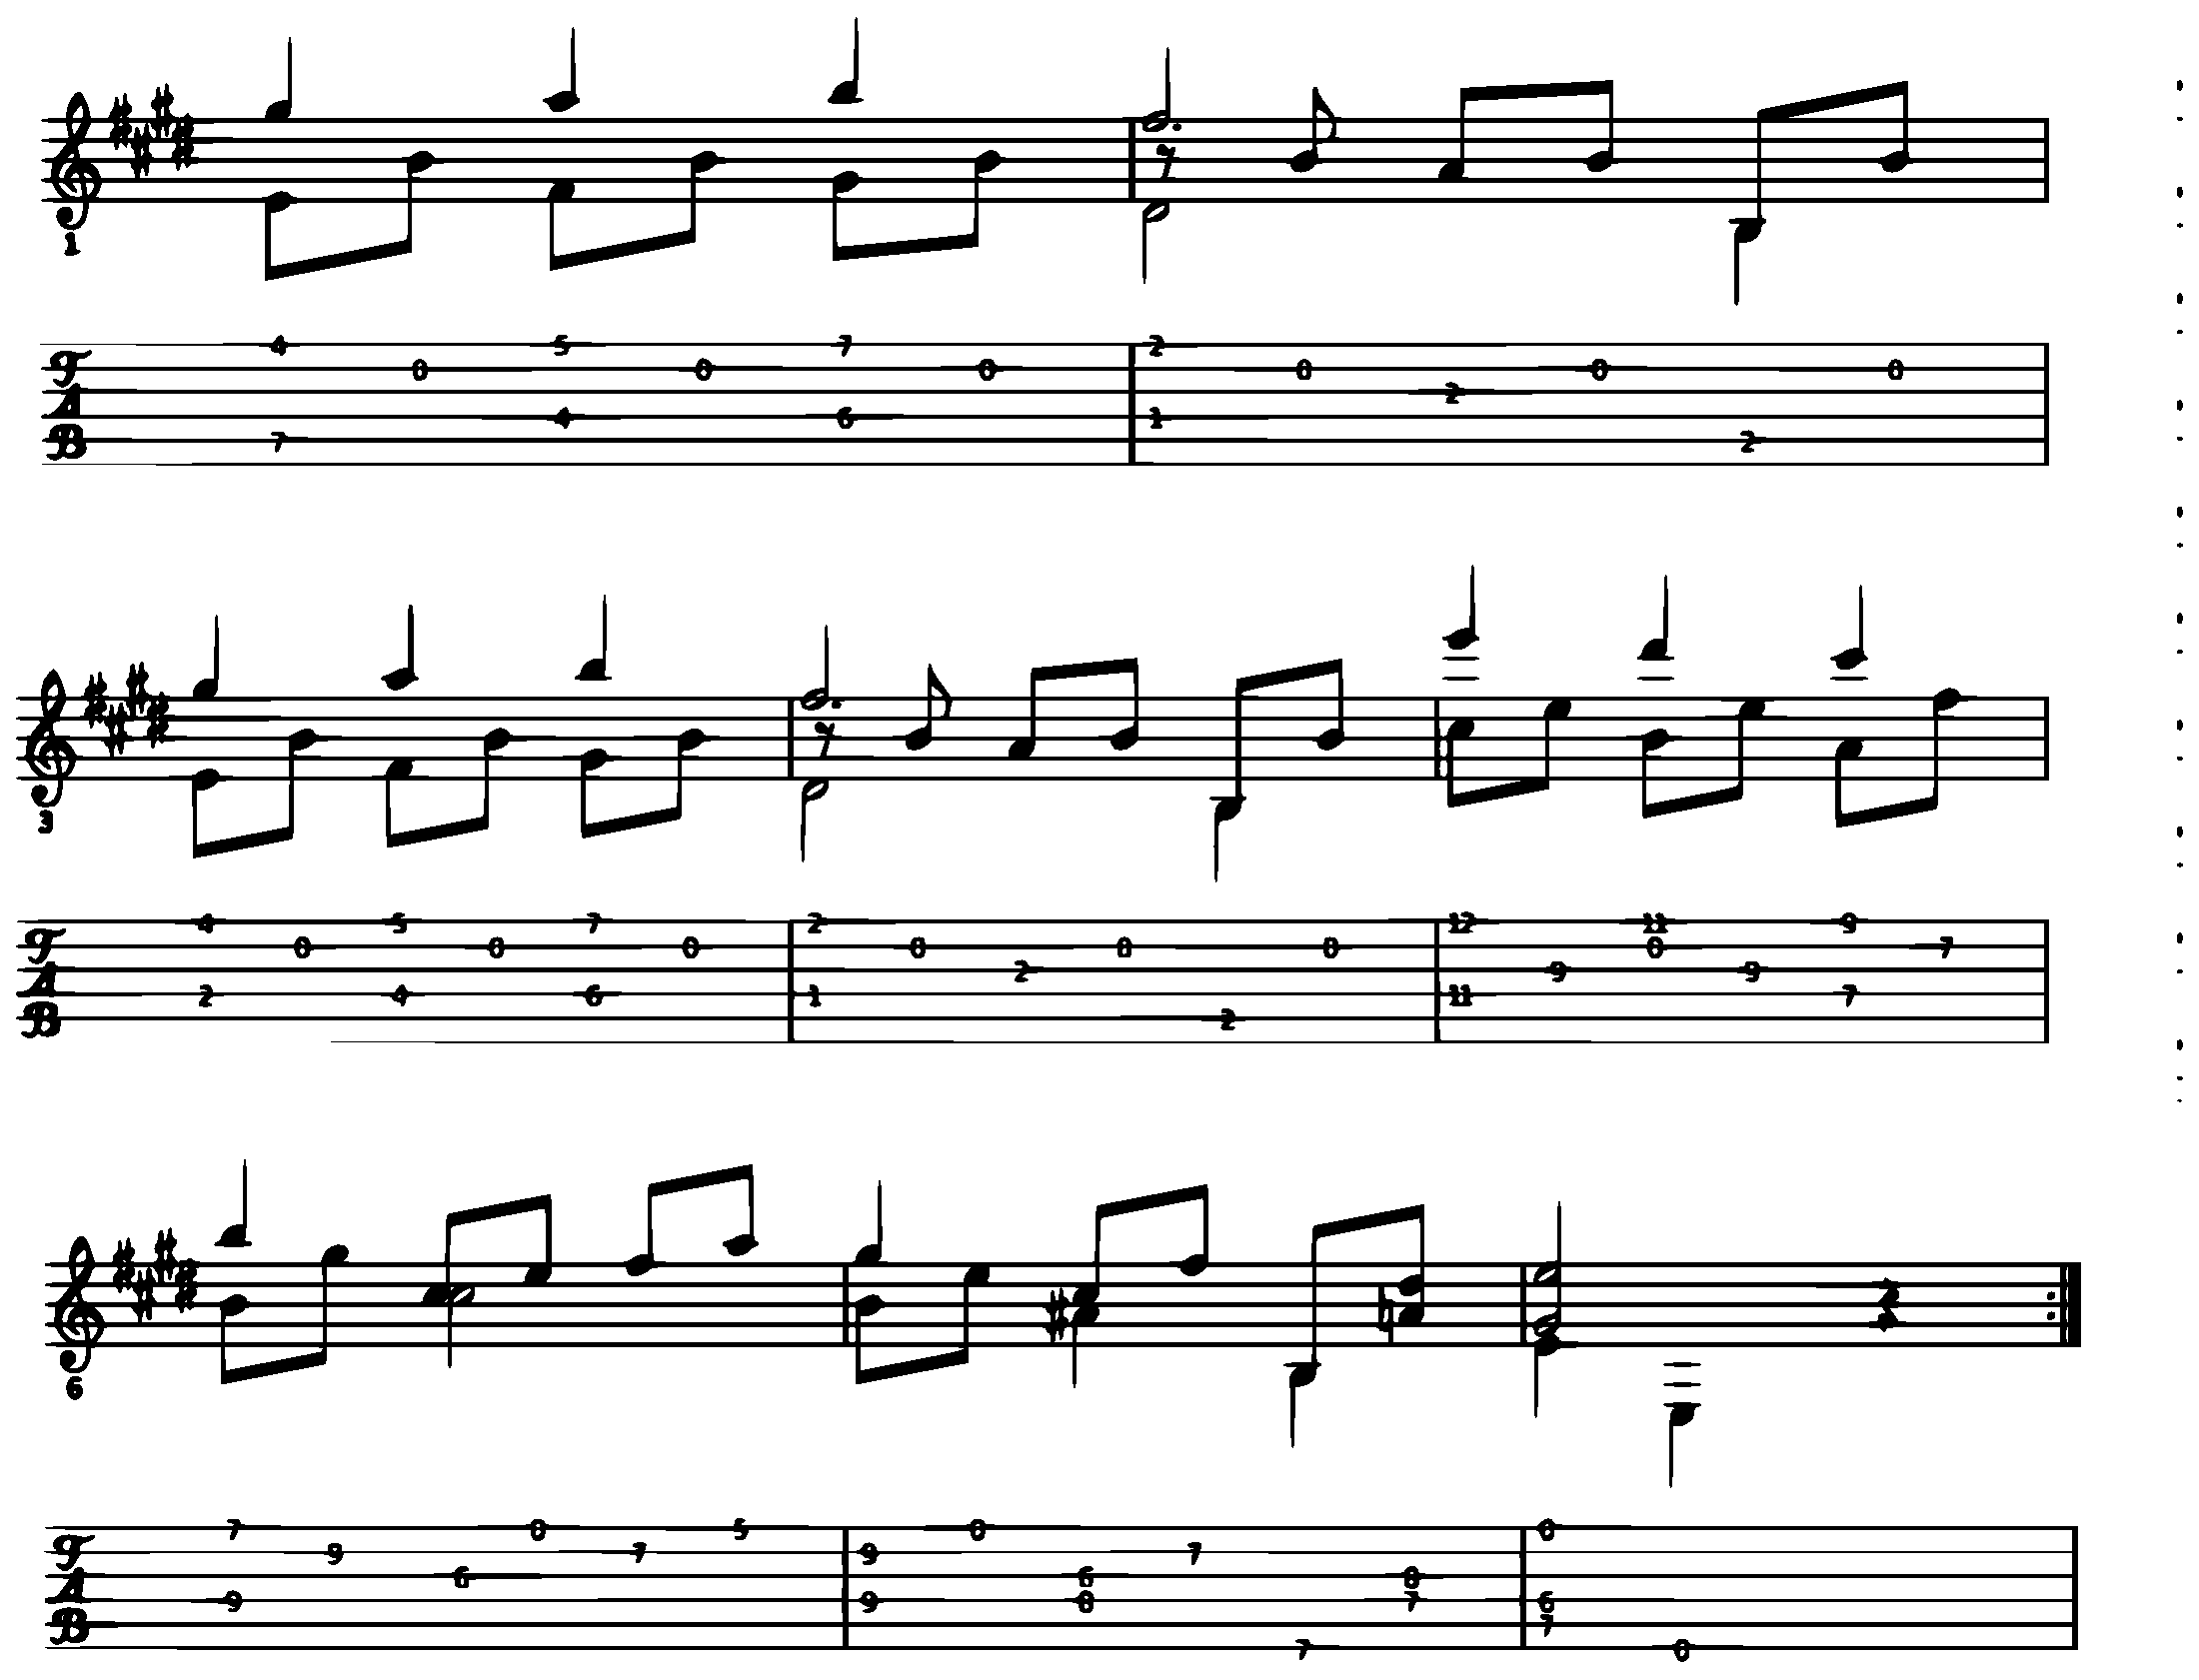
\includegraphics[width=1.0\textwidth]{Figures/Lag.eps}
    \caption{Lágrima by Francisco TÁRREGA}
    \label{fig:result-lag}
\end{figure}

\begin{figure}[h]
    \centering
    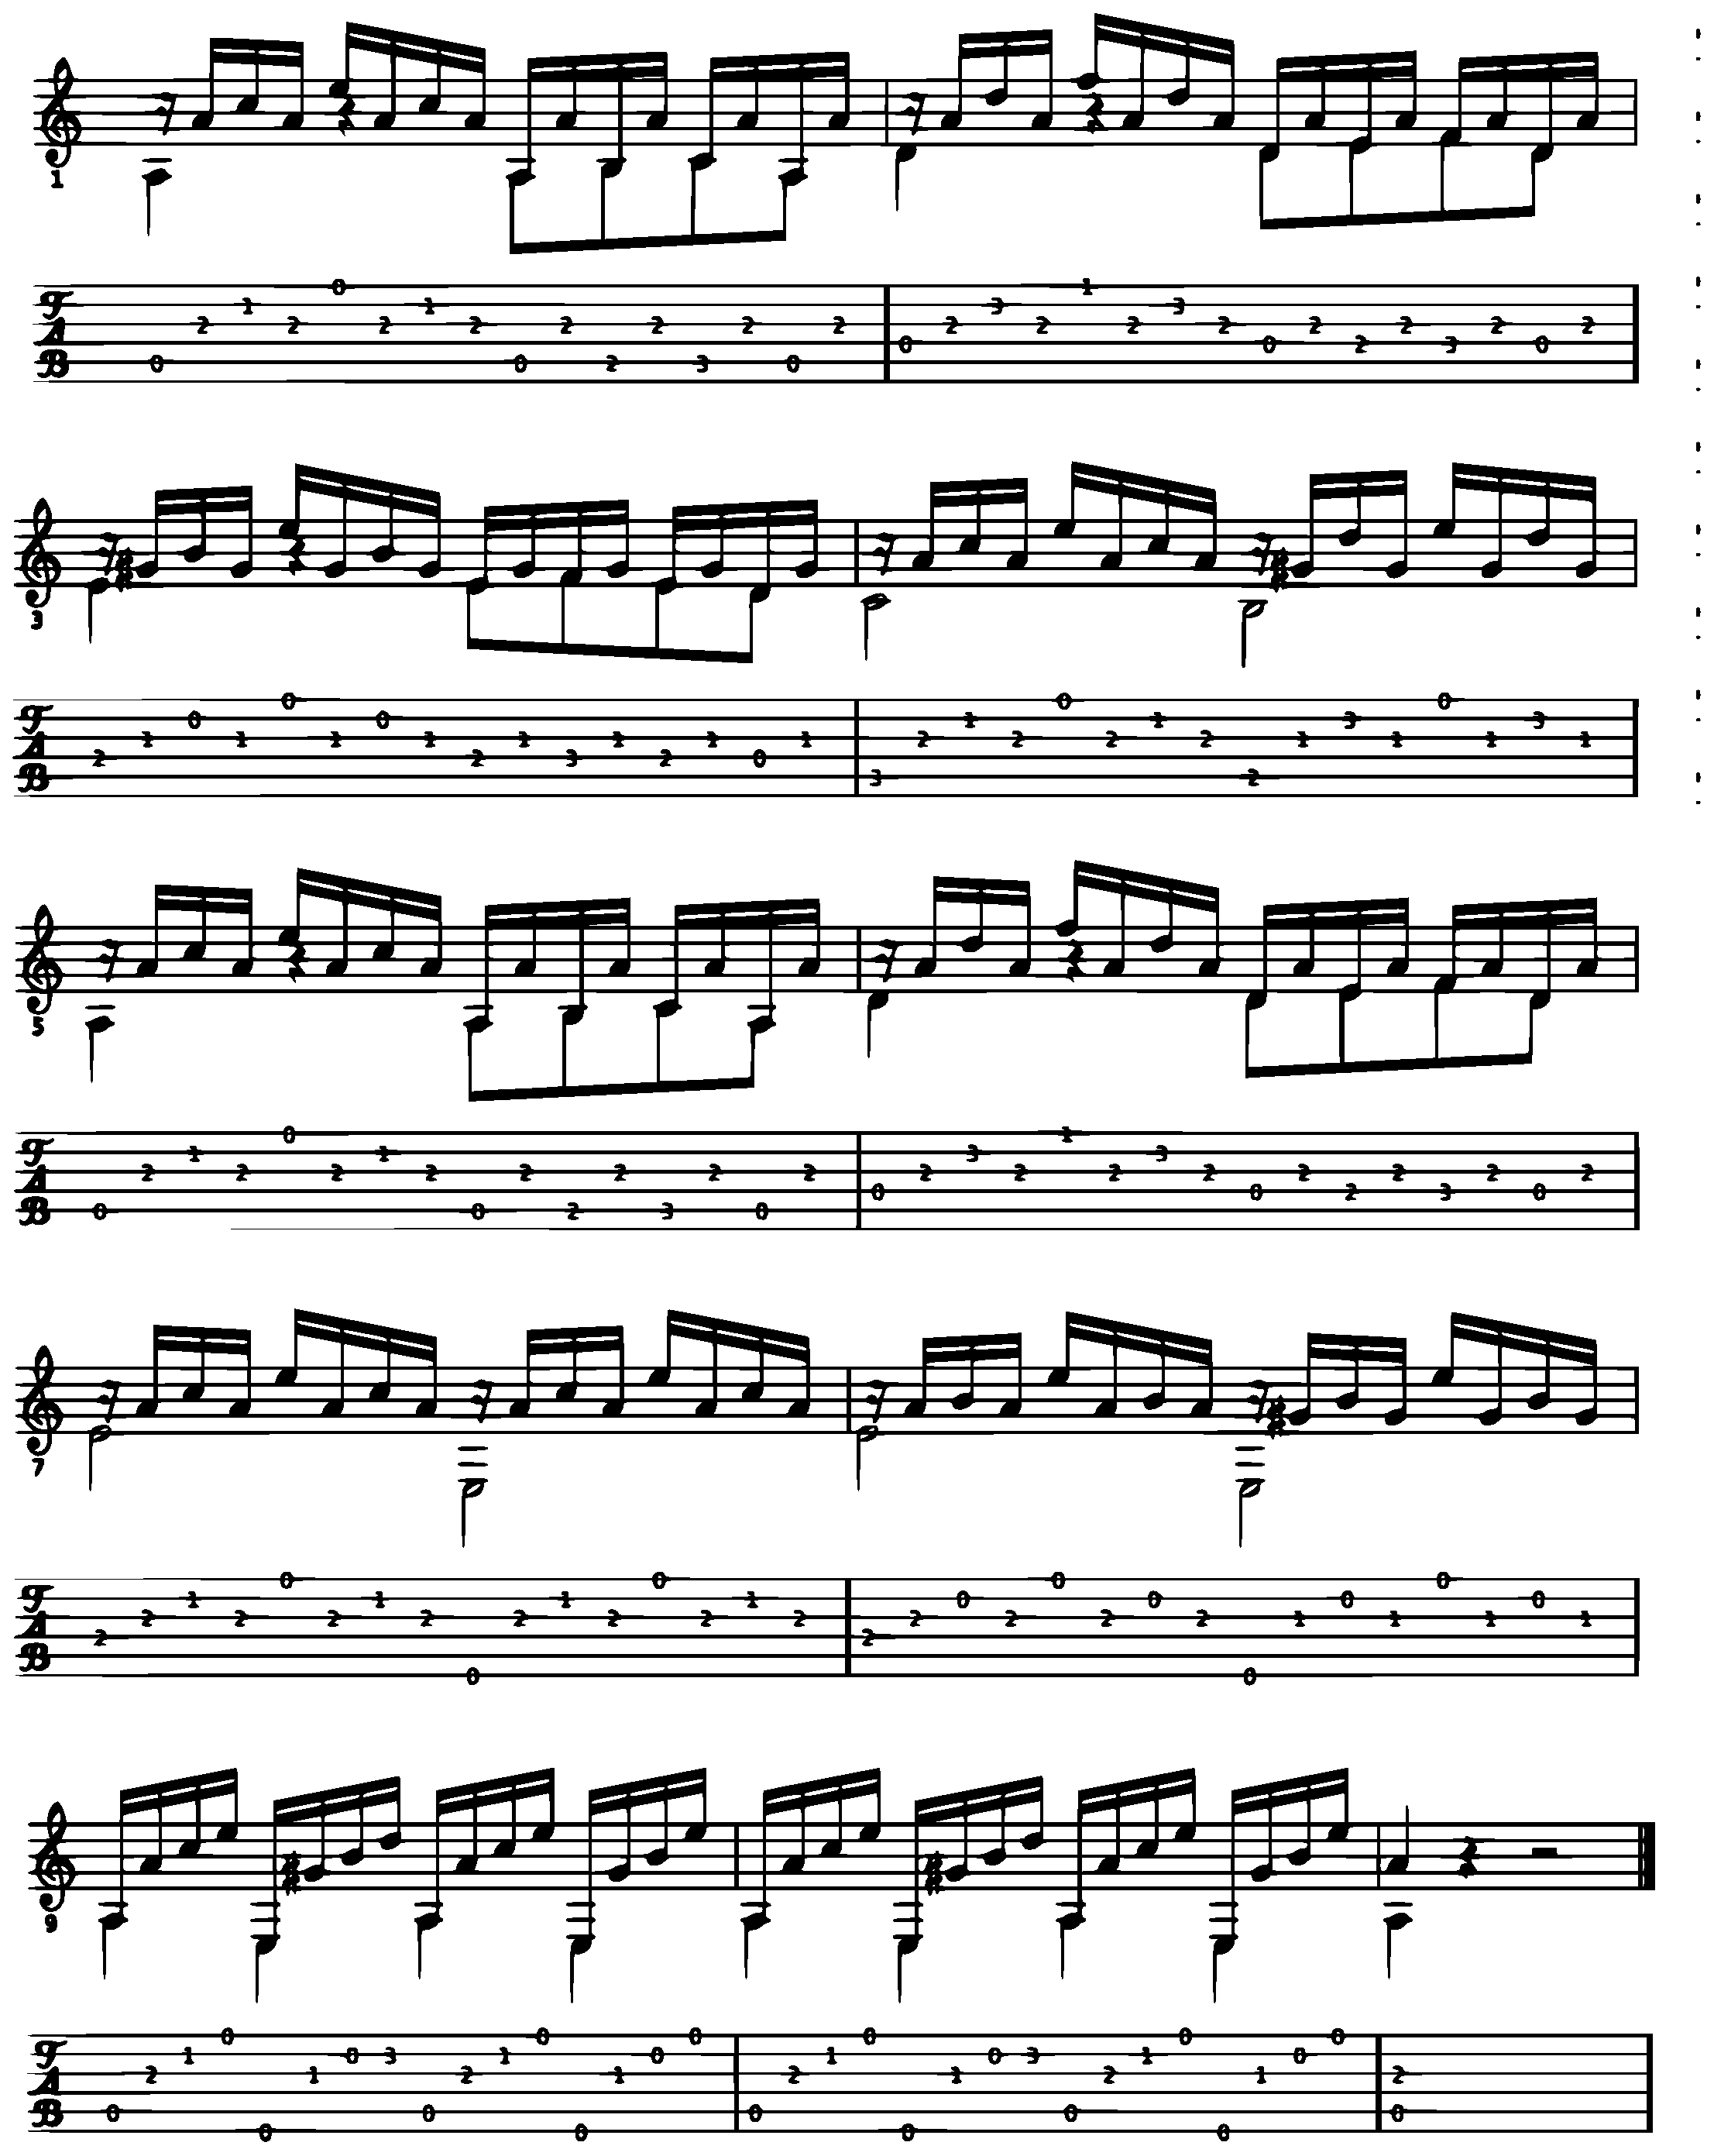
\includegraphics[width=1.0\textwidth]{Figures/Giu.eps}
    \caption{Giuliani Op.50 No.1}
    \label{fig:result-giu}
\end{figure}

\begin{figure}[h]
    \centering
    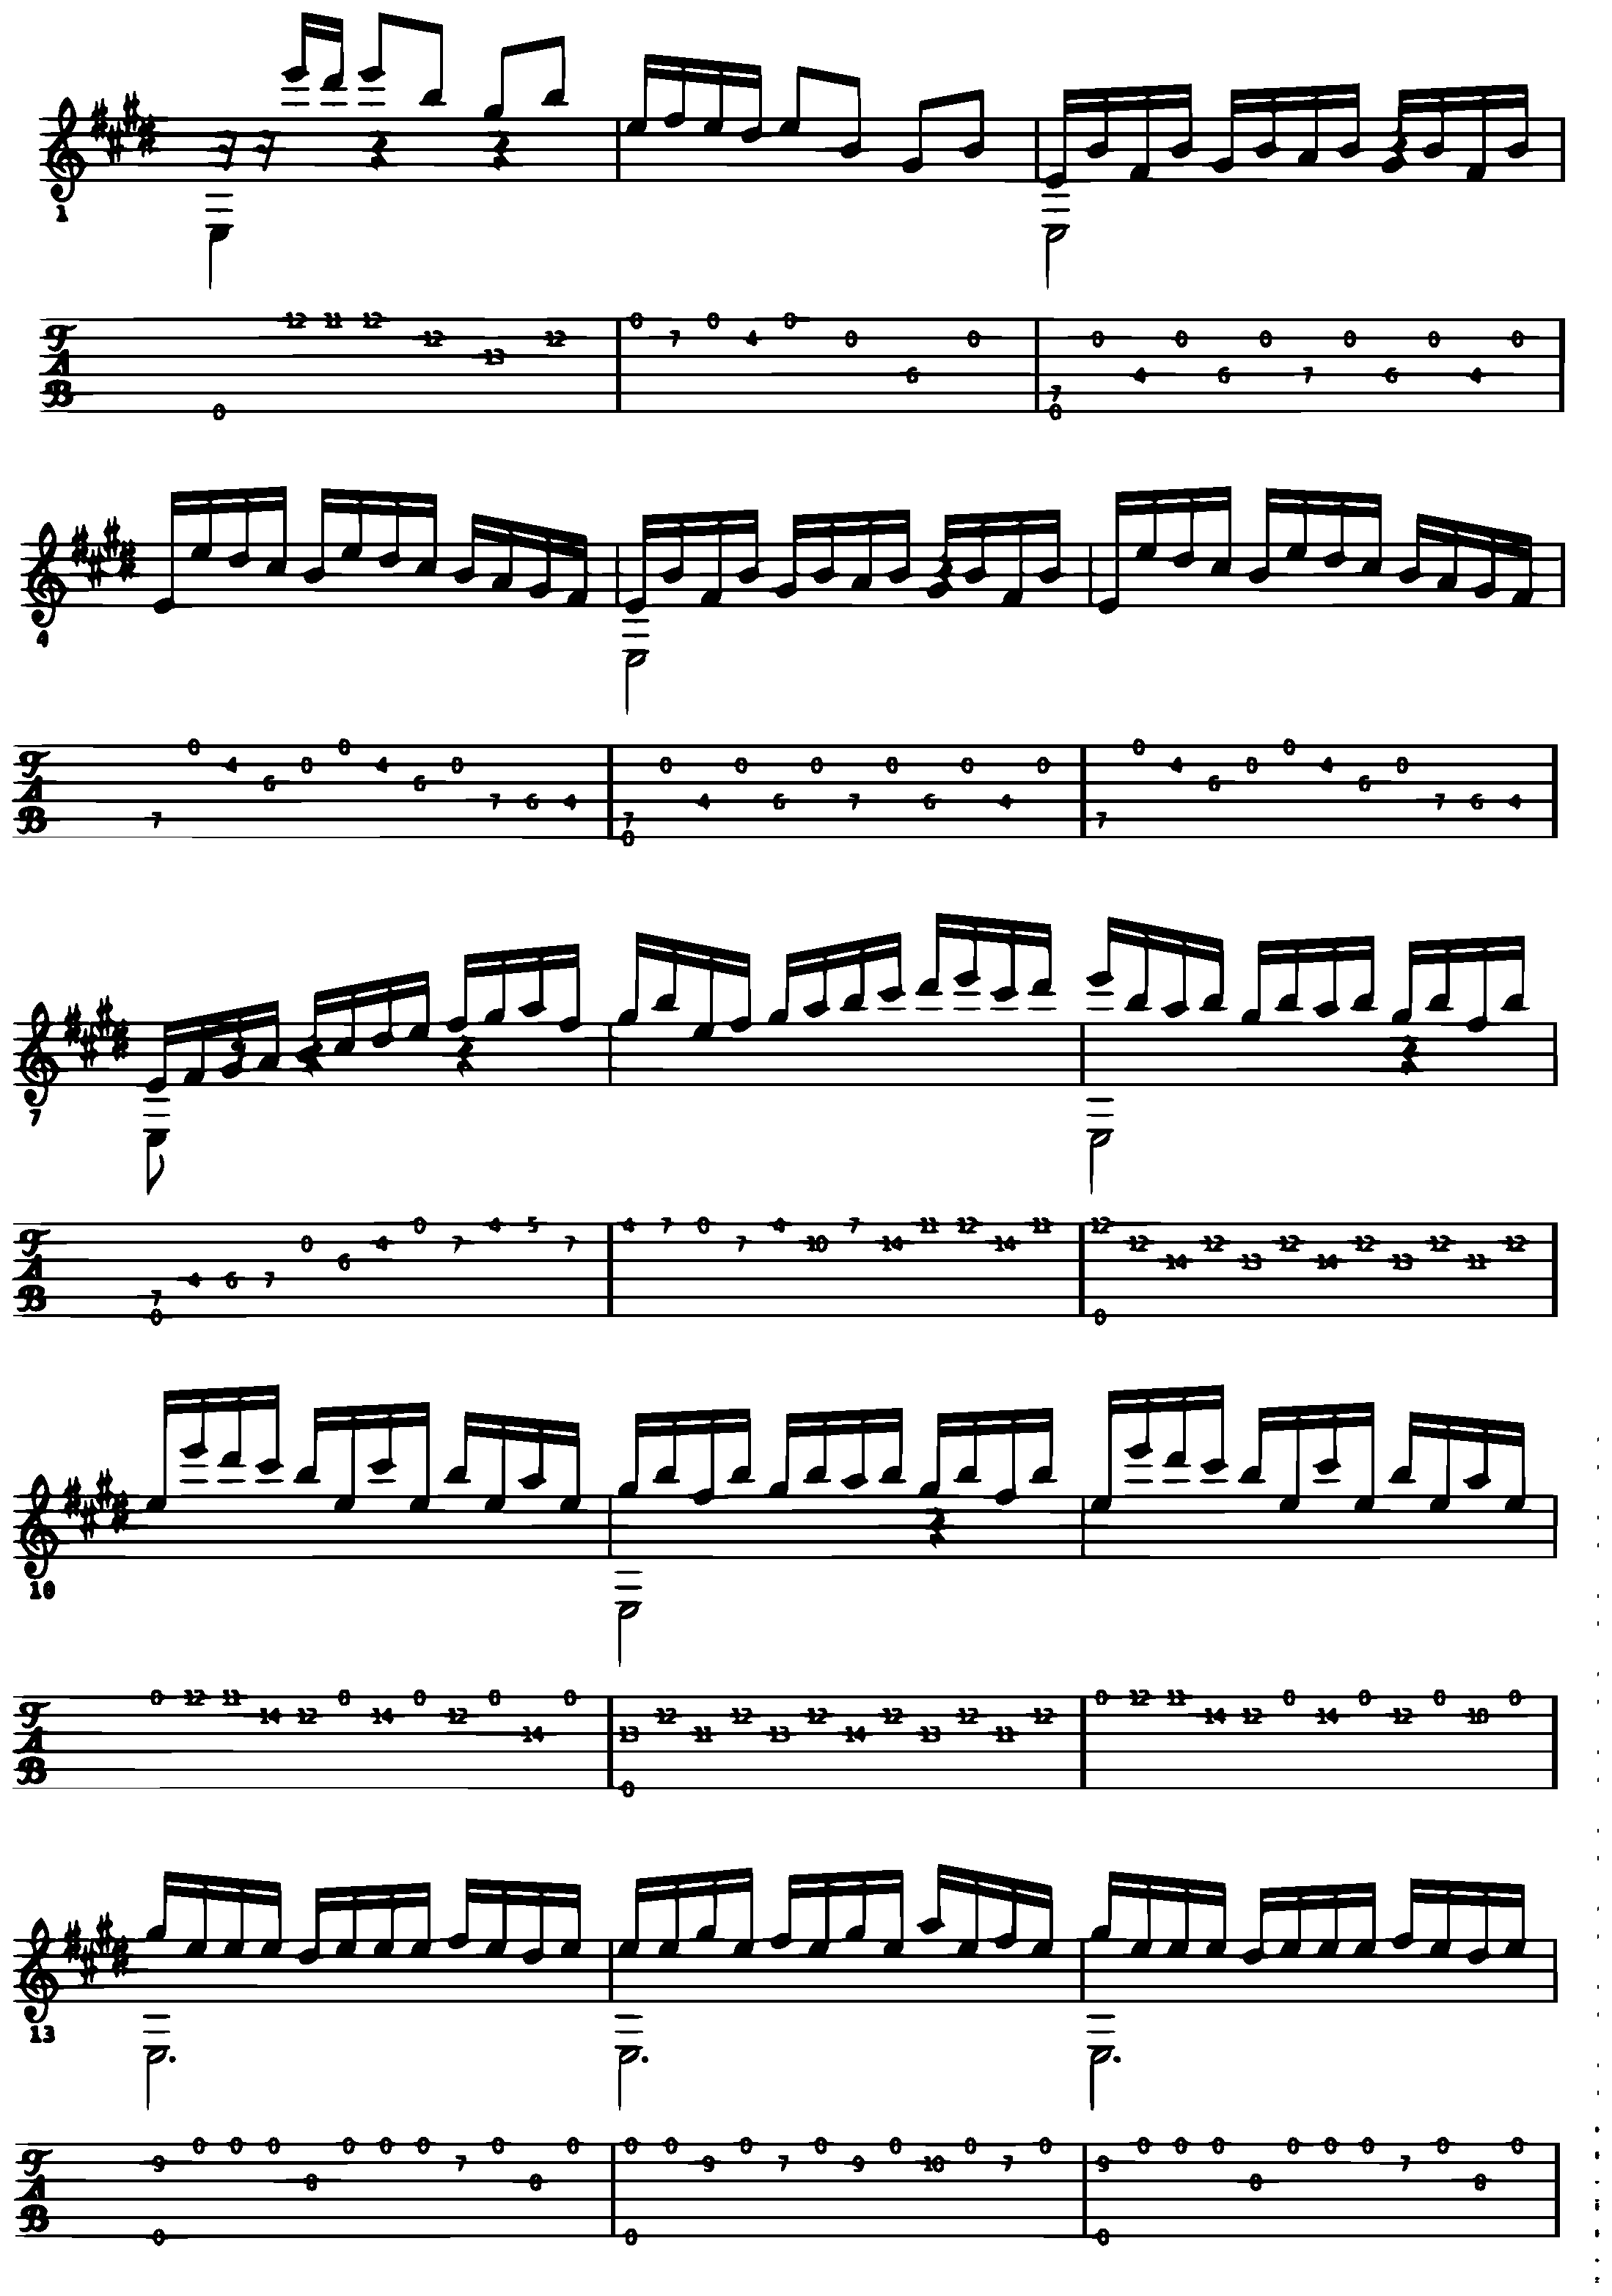
\includegraphics[width=1.0\textwidth]{Figures/Lut.eps}
    \caption{Lute Suite No.1 in E Major BWV 1006a by J.S. Bach}
    \label{fig:result-lut}
\end{figure}

\begin{figure}[h]
    \centering
    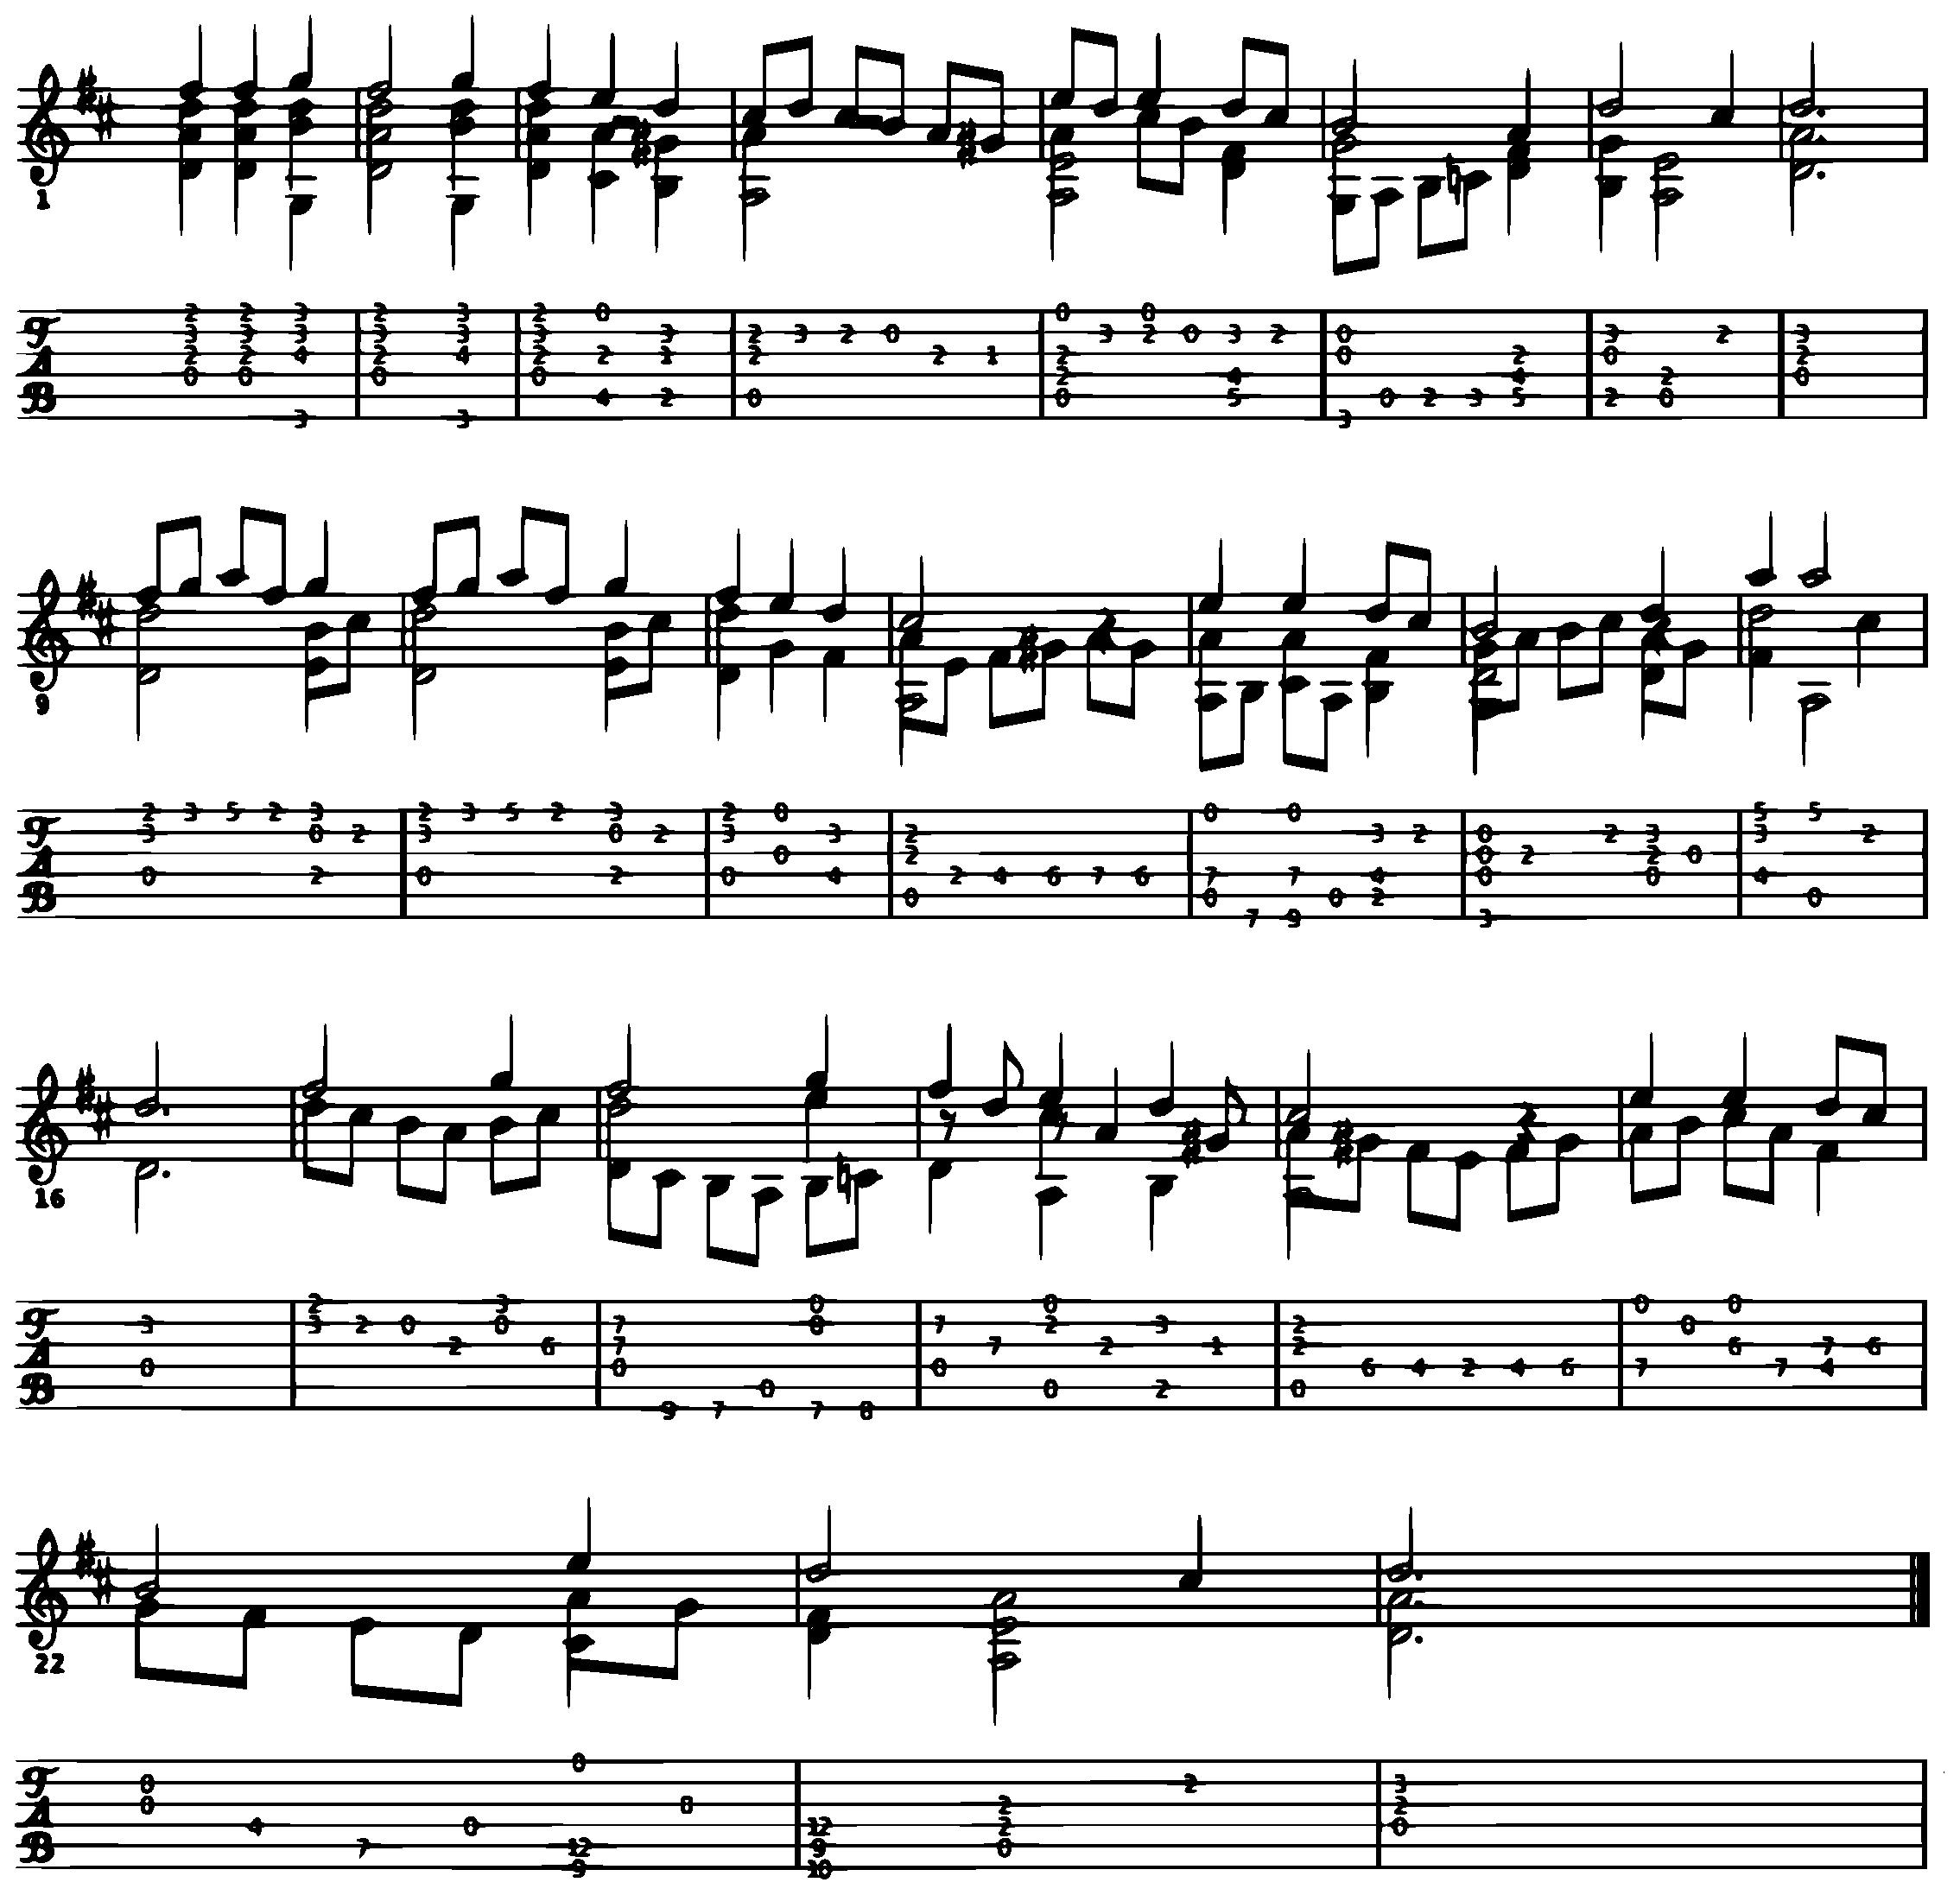
\includegraphics[width=1.0\textwidth]{Figures/Pav.eps}
    \caption{Pavane No.6 for Guitar by Luis Milan}
    \label{fig:result-pav}
\end{figure}

\chapter{Summary}

\label{Chapter:Summary}
\lhead{\emph{Summary}}

In the previous chapters, we described the most significant works in our application.

The first problem we solved is
rendering of sheet music. Scores are read from MusicXML file, which provide the necessary information for rendering.
However, not all information is given directly. Some information are context relevant and some need to be inferred by
conventional rules. 
The most challenging part of the rendering problem is to determinate the slope and stacking for beams. It is solved b
y sorting and iterating techniques. At last we got quite pleasing results.

Having audio playback in musical applications is always helpful.
The second problem we solved is playing sounds. The most important step is to generate the note sequence from the score.
The generated note sequence is also used to solve the fingering arrangement problem. 

The next problem we solved is the fingering arrangement problem. We proposed a expressive model and than used dynamic programming 
to solve the problem. The most challenging part of this method is to calculate the cost functions. We set up essential rules to 
formulate the calculation of cost functions. In the cost model we have several parameters that were unknown at the beginning. They 
are found out by experiment later. The results we got are usually properly arranged and playable. However, they are not always the  
same with the published version. It is due to that the rules in our cost model can not reflect some conventions.

To further improve the work, we should add tie note and special playing techniques to the model.
Special techniques such as hitting, picking and sliding may affect the fingering arrangement. Taking them into our model can improve
the fingering arrangement result.

% \include{Chapters/Summary}

%----------------------------------------------------------------------------------------
%	THESIS CONTENT - APPENDICES
%----------------------------------------------------------------------------------------

\addtocontents{toc}{\vspace{2em}} % Add a gap in the Contents, for aesthetics

\appendix % Cue to tell LaTeX that the following 'chapters' are Appendices

% Include the appendices of the thesis as separate files from the Appendices folder
% Uncomment the lines as you write the Appendices

\chapter{Setup Instruction}
\label{Appendix:Setup-Instruction}
\lhead{\emph{Setup Instruction}}


\addtocontents{toc}{\vspace{2em}} % Add a gap in the Contents, for aesthetics

\backmatter

%----------------------------------------------------------------------------------------
%	BIBLIOGRAPHY
%----------------------------------------------------------------------------------------

\label{Bibliography}

\lhead{\emph{Bibliography}} % Change the page header to say "Bibliography"

\bibliographystyle{unsrtnat} % Use the "unsrtnat" BibTeX style for formatting the Bibliography

\bibliography{Bibliography} % The references (bibliography) information are stored in the file named "Bibliography.bib"

\end{document}  
